\chapter{Pre-Survey and Experiment Findings}
The following chapter will give an overview of the data obtained from the survey, which was conducted before running the experiment.
Later, an overview of the data obtained from the experiment is explained along with feedback received from the participants. This chapter puts forth
all that was learnt from the above mentioned.

\section{Overview of the Pre-Survey Data}
The survey had 199 participants. Participants were not given any incentives to participate. After filtering out spurious and half-filled entries 189 entries are used for the data analysis. In the following paragraphs information obtained in the survey will be introduced.

Out of the total
participants 63.64\% are male and 36.36\% are female. The mean birth year was found to be 1985. The demographics of the participants is explained in table \ref{tab:demo}. On the education level 2.53\% have not completed high school, 9.60\% have completed high school, 5.05\% have gone to some college, 28.79\% have obtained their bachelors degree, 39.90\% have obtained their masters degrees and 14.14\% have obtained their PHDs. About the employment of the participants 51.52\% are full time employees, 6.06\% are part time employed, 6.06\% are unemployed and looking for work, 1.52\% are unemployed and not looking for work, 0.51\% are retired and 41.92\% are students. None of the participants are disabled. 

Figure \ref{fig:pre_q6} depicts the various kinds of applications the population has on their mobile phones. As seen, the most popular applications are social networking, transportation and music applications. Plot \ref{fig:pre_q7} shows the frequency of mobile usage among the population. It is observed that the majority of the people use their phones 36-70 times a day.

\begin{figure}[htp]
\subtop[Applications in the Mobile Phone\label{fig:pre_6}]{\includegraphics[width=0.45\linewidth]{./images/pre_6}}\hspace{1em}
\subtop[Mobile concern and Incentives\label{fig:pre_q15}]{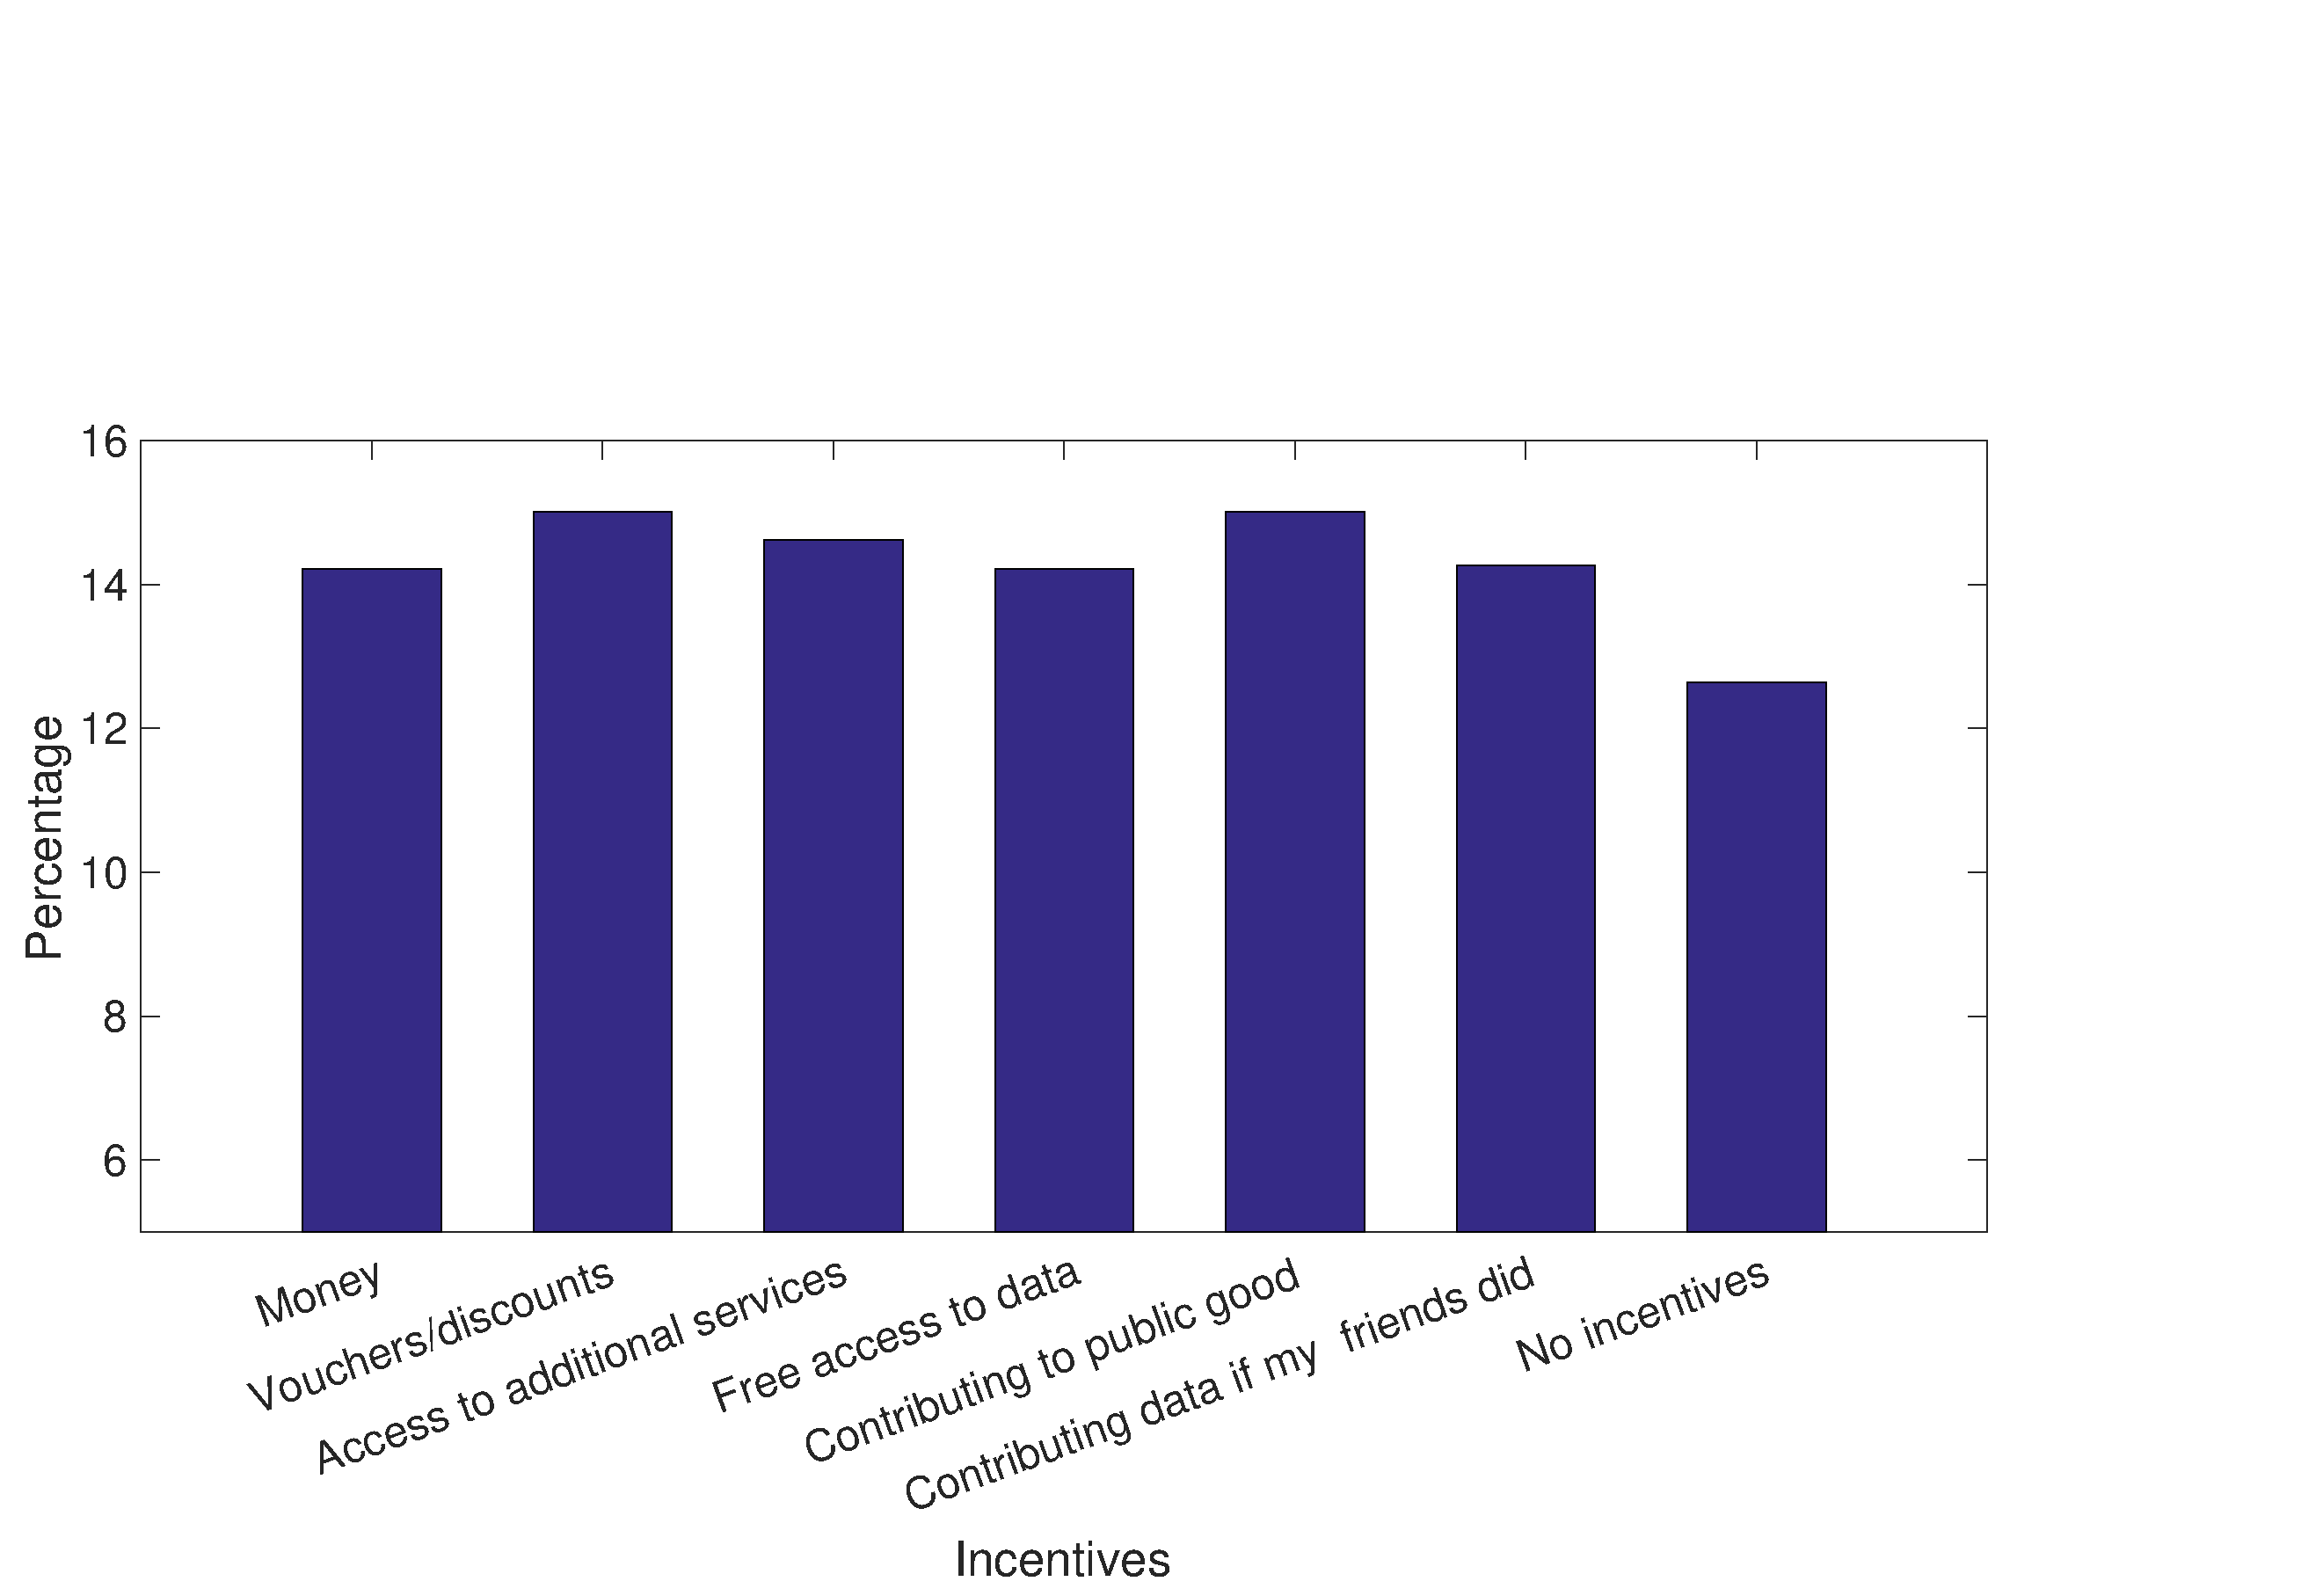
\includegraphics[width=0.45\linewidth]{./images/pre_incentives}}
\caption{Table Schemas}
\label{fig:s3}
\end{figure}

In figure \ref{fig:pre_q8}, the bars with the color dark blue represents for each level the percentage of participants. The scale of the levels are from one to five, one indicates that people do not care to five indicating that people care a lot about mobile sensor data. As observed, most people have answered level 3, meaning they care to a medium level and 77.28\% care to a level of 3 and above.

In the same figure, the color light blue shows the amount of contribution that sensors in general have in the data sharing decision. Level one indicates that it contributes none, level 5 means that it contributes a lot. It is observed that most people find that sensors contribute to a level of 4. Similarly, the color green shows the amount of contribution stakeholders in general have in the data sharing decision. It can be observed that most people find that it contributed to a level of 4. Lastly, the color yellow depicts the level of contribution contexts have in the data sharing decision. Most people feel that it contributes to a level of 5.

From the above, it is understood that in general, more than the sensor, the more important thing in a data request is for what purpose the data is being collected followed by the entity to whom the data is traded with. The privacy intrusion levels of the participants for the individual different sensors, stakeholders and contexts has been explained in chapter \ref{exp}.

At the end of it all, the aim is to study the relationship between data sharing and incentives. Figure \ref{fig:pre_q15} the percentage of people that would give data for the corresponding incentives inspite of a certain percentage of mobile concern. The higher the value of the bar, higher the mobile concern and the probability that users will share data for that incentive. As seen, "No incentives" has the lowest value of around 12\%, indicating that even tough users are less concerned, least number of users would share data for free.

%\begin{figure}[ht!]
%\centering
%\includegraphics[width=\textwidth,keepaspectratio]{./images/pre_q6}
%\caption{Applications in the Mobile Phone}
%\label{fig:pre_q6}
%\end{figure}
%
%\begin{figure}[ht!]
%\centering
%\includegraphics[width=\textwidth,keepaspectratio]{./images/pre_q7}
%\caption{Frequency of Mobile Phone Usage}
%\label{fig:pre_q7}
%\end{figure}

%\begin{figure}[ht!]
%\centering
%\includegraphics[width=\textwidth,keepaspectratio]{./images/pre_q8101214}
%\caption{Graph depicting the concern of Mobile Sensor Data and the contribution of various features to the data sharing decision}
%\label{fig:pre_q8}
%\end{figure}
%
%\begin{figure}[ht!]
%\centering
%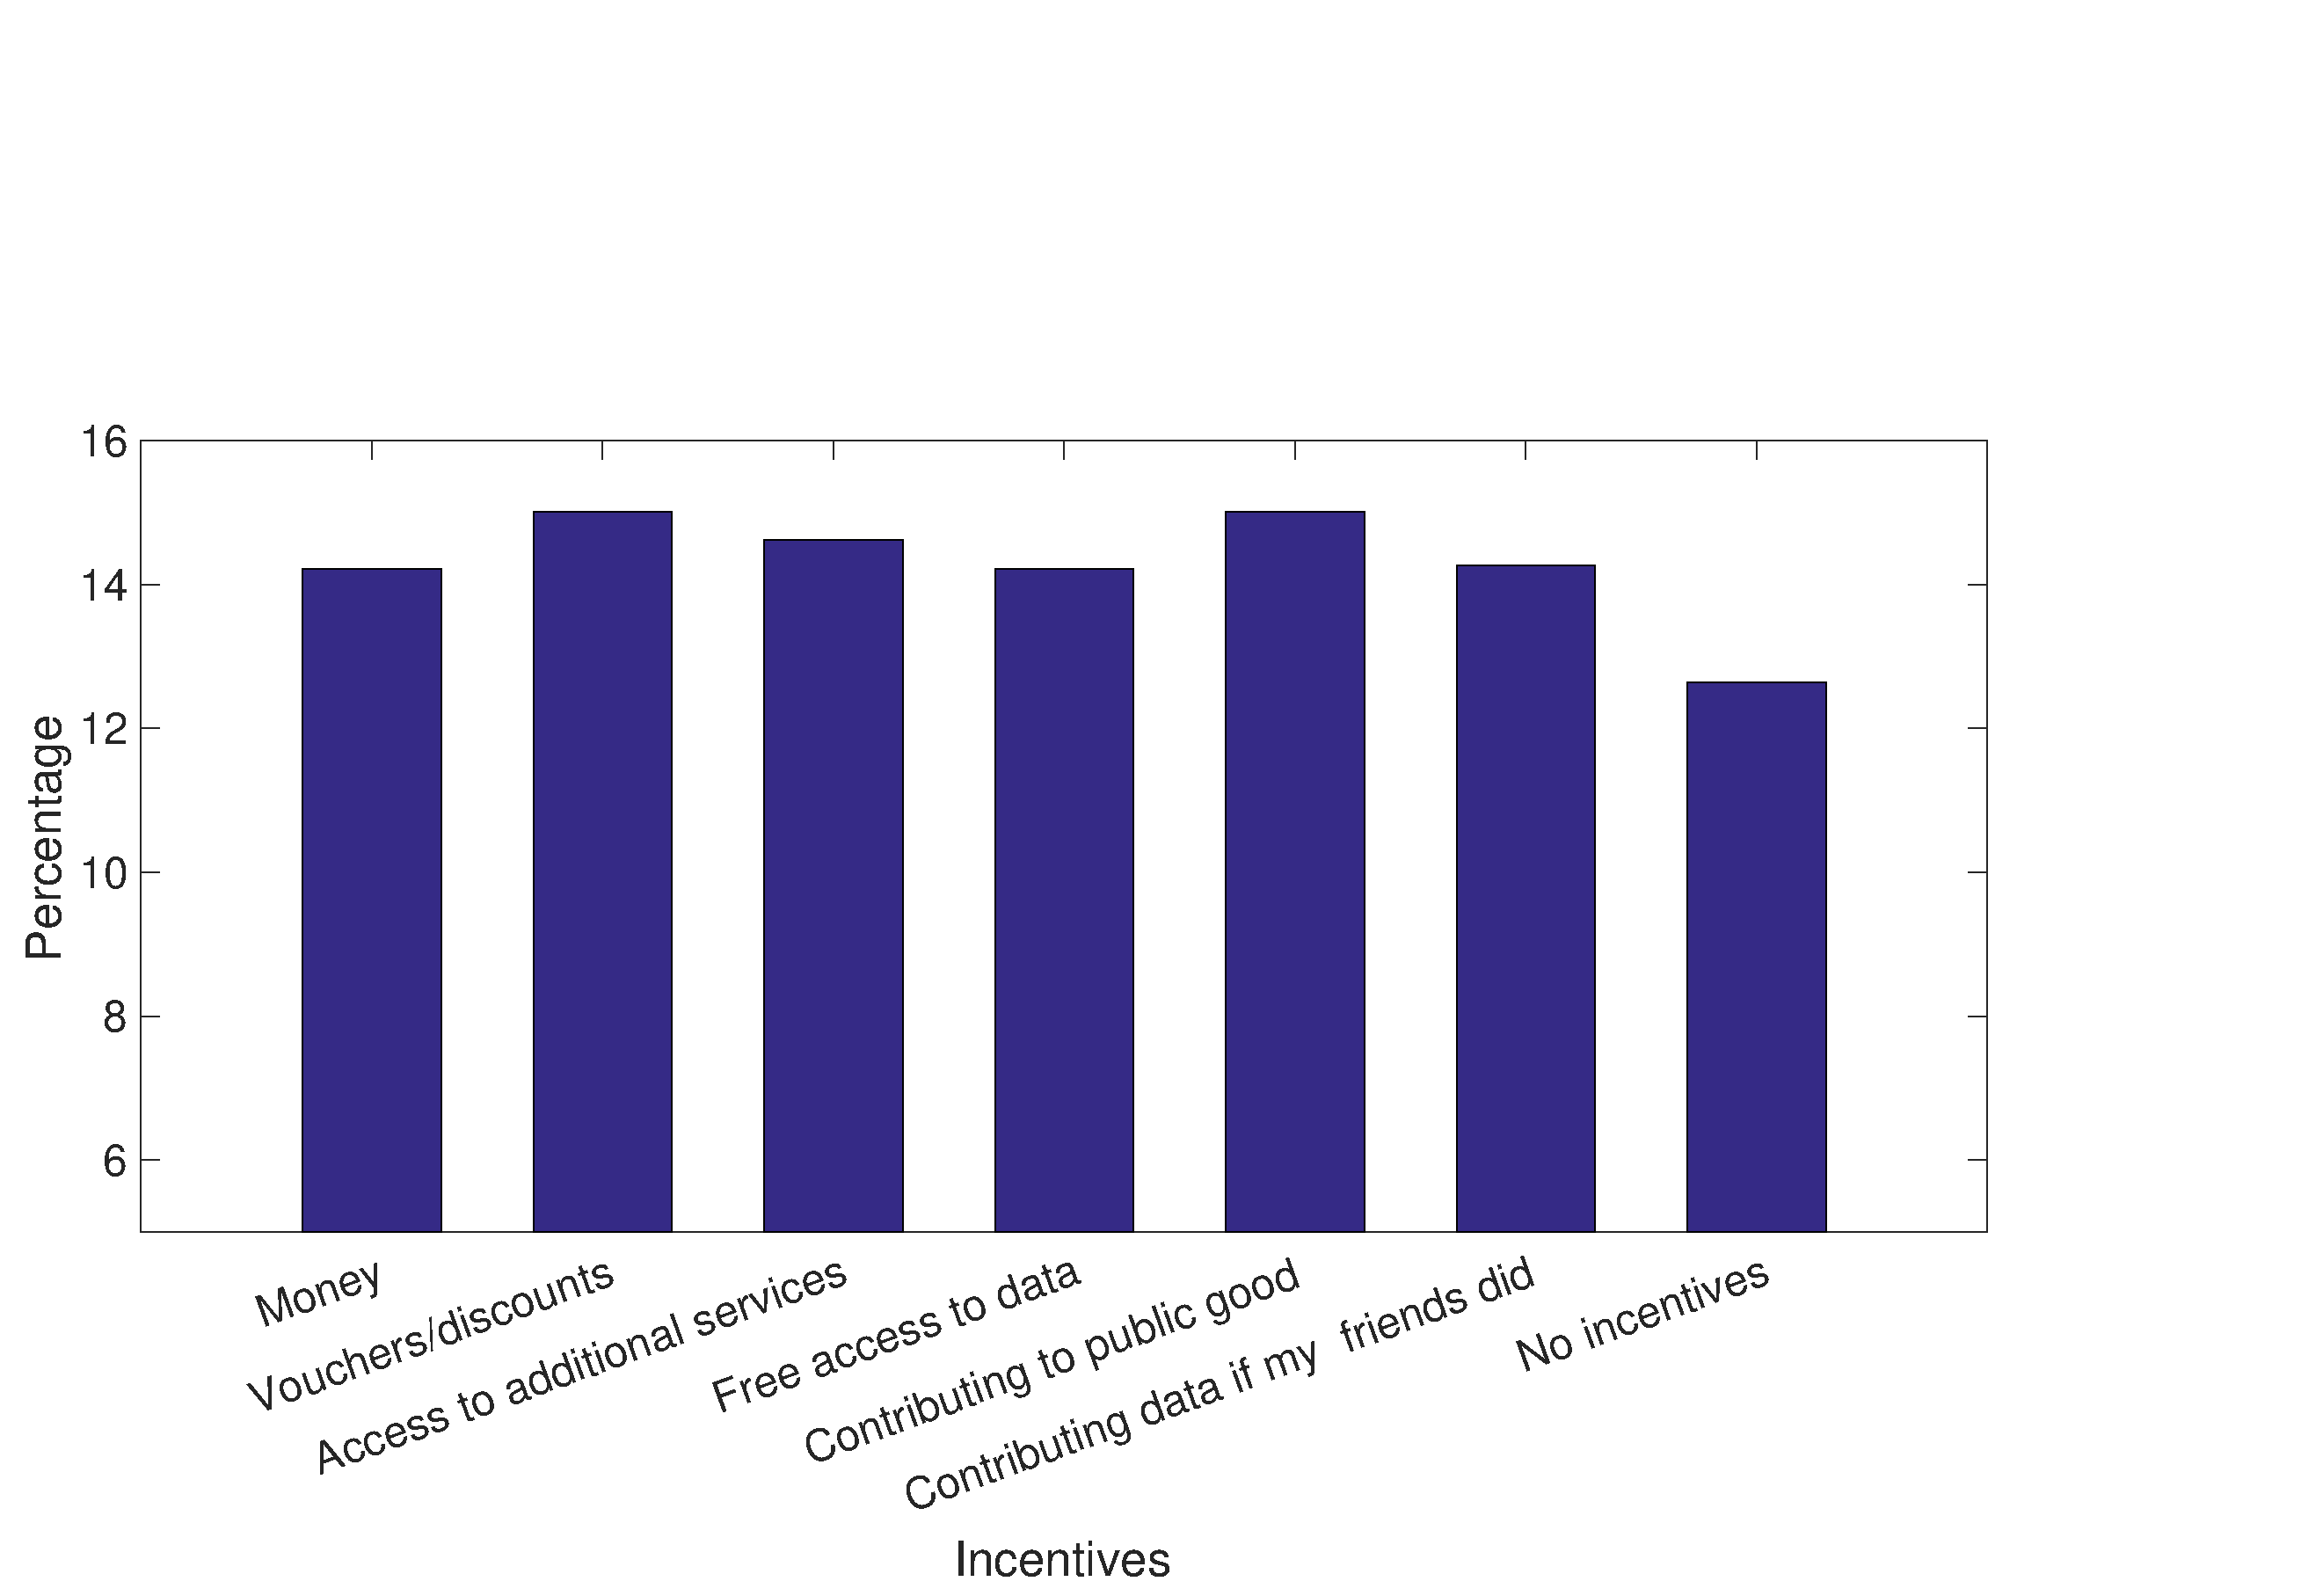
\includegraphics[width=\textwidth,keepaspectratio]{./images/pre_incentives}
%\caption{Opinions on Incentives}
%\label{fig:pre_q15}
%\end{figure}

\begin{figure}[htp]
\subtop[Graph depicting the concern of Mobile Sensor Data and the contribution of various features to the data sharing decision\label{fig:pre_q8}]{\includegraphics[width=0.45\linewidth]{./images/pre_q8101214}}\hspace{1em}
\subtop[Frequency of Mobile Phone Usage\label{fig:pre_q7}]{\includegraphics[width=0.45\linewidth]{./images/pre_q7}}
\caption{Table Schemas}
\label{fig:s3}
\end{figure}


\section{Pre-Survey Methodology and Findings}
All the results presented below were performed on the data by performing the following changes to the data:
\begin{enumerate}
\item Rows with empty fields were removed
\item Rows with spurious data were removed
\item Data was scaled or normalized when necessary
\end{enumerate}

Other than the above, the data was not manipulated. Outliers were not excluded either.

\subsubsection{Perception of Individual Sensor Grouped on the Intrusion of Sensors in General} \label{result:sensor}
W to examine here if the perception of intrusion of Sensors in general can affect the way a person views the individual sensors themselves. In other
words, we try to examine if there is a significant difference in perception of each sensor depending on the perception of the Sensors as a whole.
For this, we grouped the survey data based on the responses to question 10, which examines the contribution of sensors in general for a data request. Since there are 5 possible responses to this question, this makes 5 individual groups from 1 to 5.

The reason why this is necessary is because, if users who view Sensors in general view in the same all the individual sensor sub-features, there would be no need to ask users to individually categorize each sub-feature, a profile can be formed just based on feature categorizations.

Five groups of users are formed from one to five, who view Sensors as a whole with different intrusion levels and their perception of each of the individual sensors is now compared. Before going into the comparison, we try to understand the properties of the data to analyze. Essentially, we try to examine if each of the groups formed come different populations and for this the most popular statistical tests are the T-test and the one-way ANOVA. To perform a one-way ANOVA test or a T-test, the data should be\footnote{\url{https://fr.wikipedia.org/wiki/Analyse\_de\_la\_variance}}:

\begin{enumerate}
\item Normally distributed
\item Homoscedastic
\item Ordinal or continuous
\end{enumerate}

Since the data of the survey is discrete and follows the Likert Scale with options from 1 to 5, it gives skewed normal distribution. The scale used to collect data is in the ordinal form. Additionally, the variances of values within the groups formed are not similar. The one-way ANOVA test is quite robust to heteroscedacity, as long as the maximum variance among all groups is less than four times the group with the lowest variance.  Accounting for all the violations, we instead opt for non-parametric tests such as the Kruskal-Wallis H-test and the Dunn's test
which only assume the following\footnote{\url{https://en.wikipedia.org/wiki/Kruskal-Wallis\_one-way\_analysis\_of\_variance}} : 

\begin{enumerate}
\item Groups are independant from one another
\item All observations are independant
\item The dependant variables should be in the ordinal scale or continuous
\end{enumerate}

The above tests do not make any assumptions about the distribution of the data and are robust to heteroscedastic data.
\begin{figure}[htp]
\subtop[Mean of each Group for each Sensor\label{fig:s1}]{\includegraphics[width=0.5\linewidth,height=0.45\linewidth]{./images/sensors_group_meanQ10}}
\subtop[Variance of each Group for each Sensor\label{fig:s2}]{\includegraphics[width=0.5\linewidth,height=0.45\linewidth]{./images/sensors_group_varianceQ10}}
\caption{Table Schemas}
\label{fig:s3}
\end{figure}

Group 1 to 5 which consist of users with different perception of Sensors have 13, 14, 50, 71 and 42 people in each group respectively. For in depth information of the composition of each group in terms of employment, education, gender and birth year please refer to tables
\ref{tab:emp_sensors},\ref{tab:edu_sensors},\ref{tab:gender_sensors},\ref{tab:year_sensors}. Figures \ref{fig:s1} and \ref{fig:s2} depict the mean and variances for each of the individual groups. We start by performing the non paramteric Kruskal-Wallis test for each individual sensor. The value of alpha assumed here is 0.05. The null hypothesis states that all the groups perceive all the sensors in the similar way. This means they come from the same population. The alternative hypothesis is
that the groups perceive each sensor in a significantly different way and hence their populations are distinct. The table \ref{tab:kw_sensors} depicts the p-values obtained from the statistical test.

\begin{table}[h!]
  \centering
  \caption{Kuskal-Wallis Test For Sensors}
  \label{tab:kw_sensors}
  \begin{tabular}{cccc}
    \toprule
     Sensor & p-value \\
    \midrule
    Accelerometer & 0.0151 \\
    Gyroscope & 0.2959\\
    Location & 1.0664e-05\\
    Proximity & 0.0147\\ 
    Light & 0.6933\\
    Battery & 0.6950\\ 
    Microphone & 3.0070e-04\\
    Camera & 2.1191e-05\\
    Thermometer & 0.0693\\ 
    Air Humidity & 0.1292\\
    Barometer & 0.0949\\
    Bluetooth & 3.4877e-05\\ 
    \bottomrule
  \end{tabular}
\end{table} 

Accelerometer, location, proximity, microphone, camera and bluetooth are the sensors for which the groups opinions vary significantly.
On these sensors, we proceed with a post hoc test for further investigation by performing a pariwise Dunn's test to examine if there is an actual significant difference between the groups and if so between which groups. The sensors with p-values with less than 0.05 are examined in more detail and the p-values are presented in table \ref{tab:dunn_sensors}. The table shows the results for each pairwise test done, with the p-values adjusted using the Bonferroni Method\footnote{\url{https://en.wikipedia.org/wiki/Bonferroni\_correction}}. The reason for choosing to adjust the p-values is that repeated experiments can increase the chances of accepting the alternative hypothesis so p-values are adjusted according to the number of experiments performed. 10 experiments are performed per sensor.

For the Accelerometer and Proximity sensors, it is seen that none of the pairwise groups have a significant difference from each other. This means that even tough the groups perceive sensors differently in general, they all view Accelerometers and Proximity in a similar way. This is reinforced in figures \ref{fig:se_acc} and \ref{fig:se_prox}, where it is seen that there is significant overlap between the population of the groups.

For the location sensor, it is observed that groups (1,4), (1,5), (2,4), (2,5) have a significant difference. This can be attributed to the fact that since the groups are formed from the perception of people of the sensors feature, the difference in perception between group 1 and group 5 will be larger than between group 1, group 2 and group 1, group 3 since they are not much apart in the scale. Figure \ref{fig:se_loc} depicts the spread of the group populations for the location sensor. As found groups (1,4), (1,5), (2,4), (2,5) have the least amount of overlap.

For the microphone sensor, it can be seen that groups (1,3), (1,4) and (1,5) are significantly different from each other. This goes to show that
if people rate sensors as even a little intrusive, they all rate the microphone's in a significantly different way than the people who rate sensors as non-intrusive. Figure \ref{fig:se_micro} depicts the spread of the population of the groups.

For the camera sensor, it can be observed that groups (1,4), (1,5), (2,4), (2,5) have a significant difference in their perception of the intrusion. Similar to the location sensor, people with perception of sensors in general with a lower intrusion level have significantly different responses to the camera intrusion than the people who rate sensors with more intrusion. Figure \ref{fig:se_cam} depicts the spread of the population of the groups for the camera sensor.

For the Bluetooth sensor, there is a significant difference between groups (1,5), (2,5), (3,5) and (4,5). This shows that responses by people who find sensors extremely intrusive is different from the rest of the groups. This fact is reinforced by figure \ref{fig:se_blue} where it is seen that group 5 has least overlap with other groups.

It can be concluded that some sensors such as the accelerometer, proximity, gyroscope, light, battery, thermometer, humidity, barometer are sensors where each of the groups do not have significantly different opinions of intrusion. Sensors such as the camera, microphone, location and bluetooth
are where opinions differ between groups. These sensors are found to be on average more intrusive with intrusion values of 4.23, 3.87, 4.14 and 3.52 respectively on a scale of five. Groups with larger differences between them (such as group 1 and 4) tend to have larger differences in opinions for some sensors generally considered intrusive. Groups with smaller differences between them (such as group 1 and 2) tend to have similar opinions.

Higher incentives can be given to people for generally intrusive sensors, but the incentives should be even higher in order to motivate users from high intrusion groups (such as group 5) to give their sensor data. 


\begin{table}[h!]
  \centering
  \caption{Dunn's Test For Sensors}
  \label{tab:dunn_sensors}
  \begin{tabular}{ccccccc}
    \toprule
     Groups & Accelerometer & Location & Proximity & Microphone & Camera & Bluetooh \\
    \midrule
    (1,2) & 1.0000 & 1.0000 & 0.9992 & 0.8365 & 1.0000 & 1.0000 \\
    (1,3) & 0.4207 & 0.2084 & 0.0699 & 0.0365 & 0.0732 & 0.7825 \\
    (1,4) & 0.0595 & 0.0125 & 0.0513 & 0.0012 & 0.0048 & 0.6442 \\
    (1,5) & 0.2054 & 0.0010 & 0.1191 & 0.0009 & 0.0007 & 0.0029 \\
    (2,3) & 0.6548 & 0.1774 & 0.3713 & 0.8927 & 0.1694 & 0.5921 \\
    (2,4) & 0.1185 & 0.0077 & 0.2617 & 0.2287 & 0.0123 & 0.4270 \\
    (2,5) & 0.3659 & 0.0005 & 0.5184 & 0.1597 & 0.0018 & 0.0007 \\
    (3,4) & 0.8989 & 0.7642 & 1.0000 & 0.8052 & 0.9040 & 1.0000 \\
    (3,5) & 0.9997 & 0.0869 & 1.0000 & 0.6390 & 0.2947 & 0.0066 \\
    (4,5) & 0.9998 & 0.8360 & 1.0000 & 1.0000 & 0.9617 & 0.0059 \\
    \bottomrule
  \end{tabular}
\end{table} 

\begin{figure}[htp]
\subtop[Accelerometer\label{fig:se_acc}]{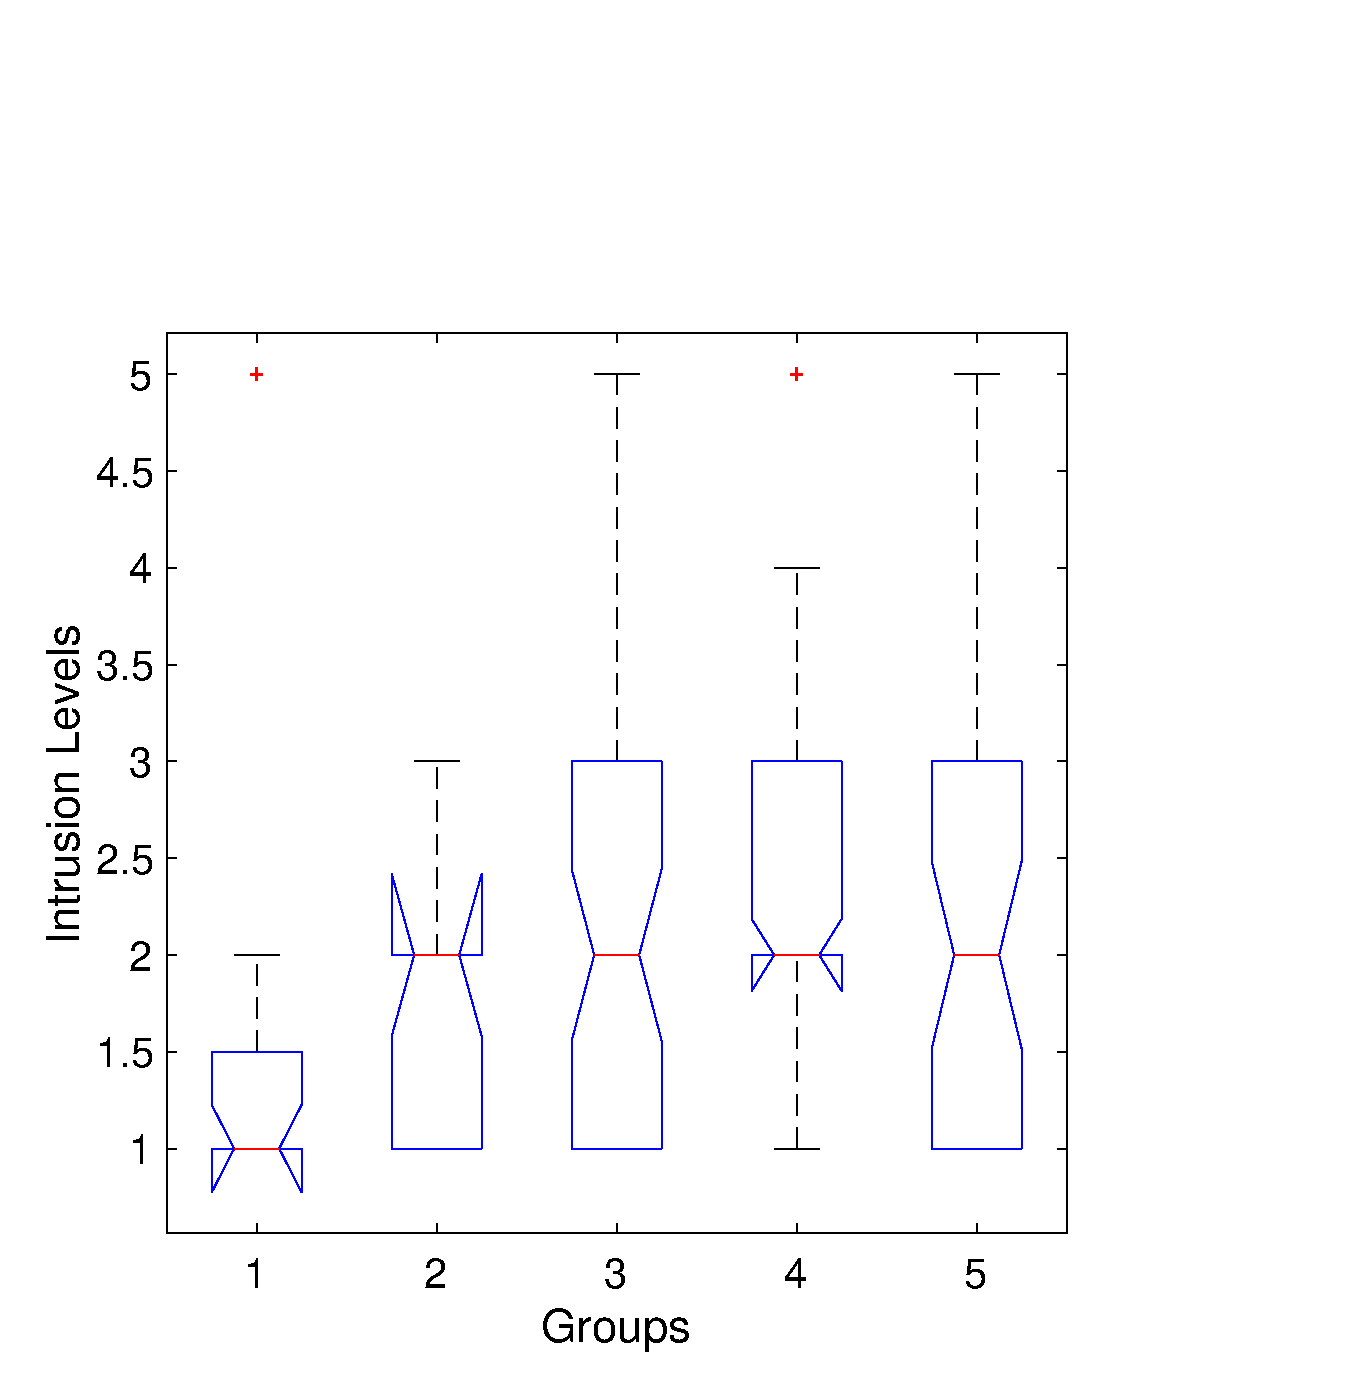
\includegraphics[width=0.45\linewidth]{./images/acc_box}}\hspace{1em}
\subtop[Location\label{fig:se_loc}]{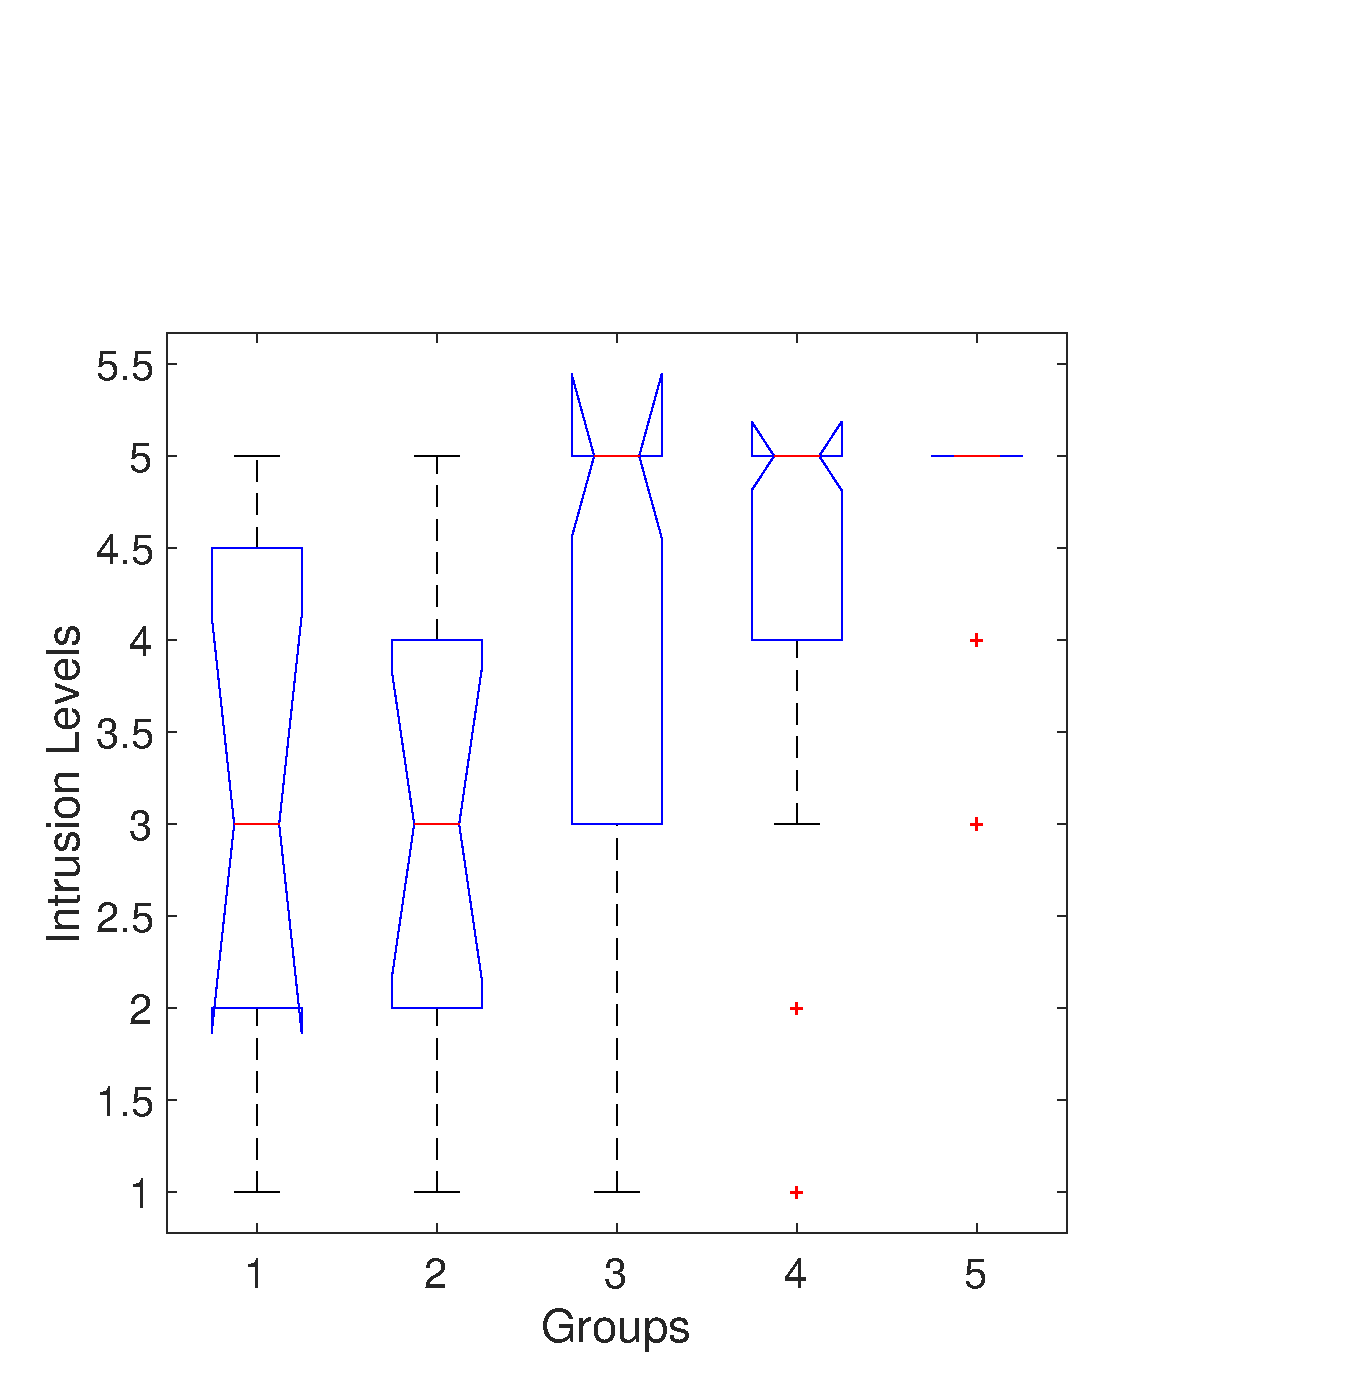
\includegraphics[width=0.45\linewidth]{./images/loc_box}} \newline
\subtop[Proximity\label{fig:se_prox}]{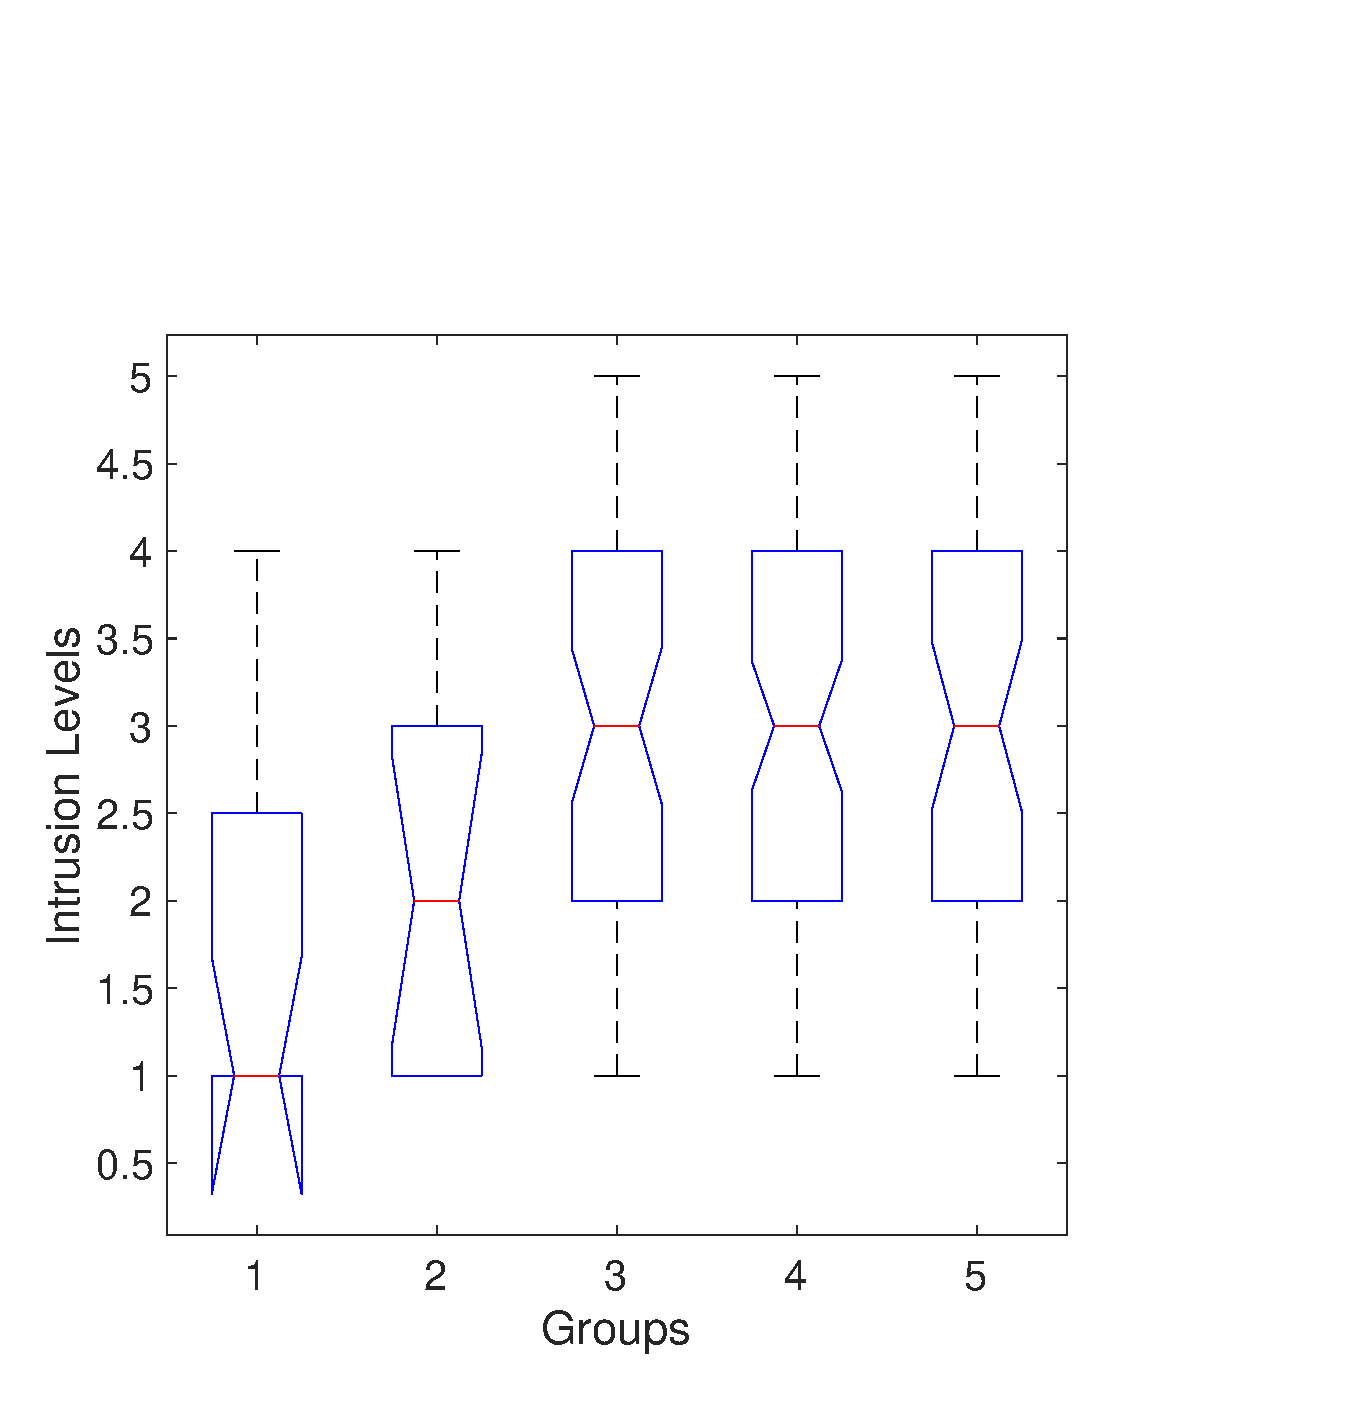
\includegraphics[width=0.45\linewidth]{./images/prox_box}}\hspace{1em}
\subtop[Microphone\label{fig:se_micro}]{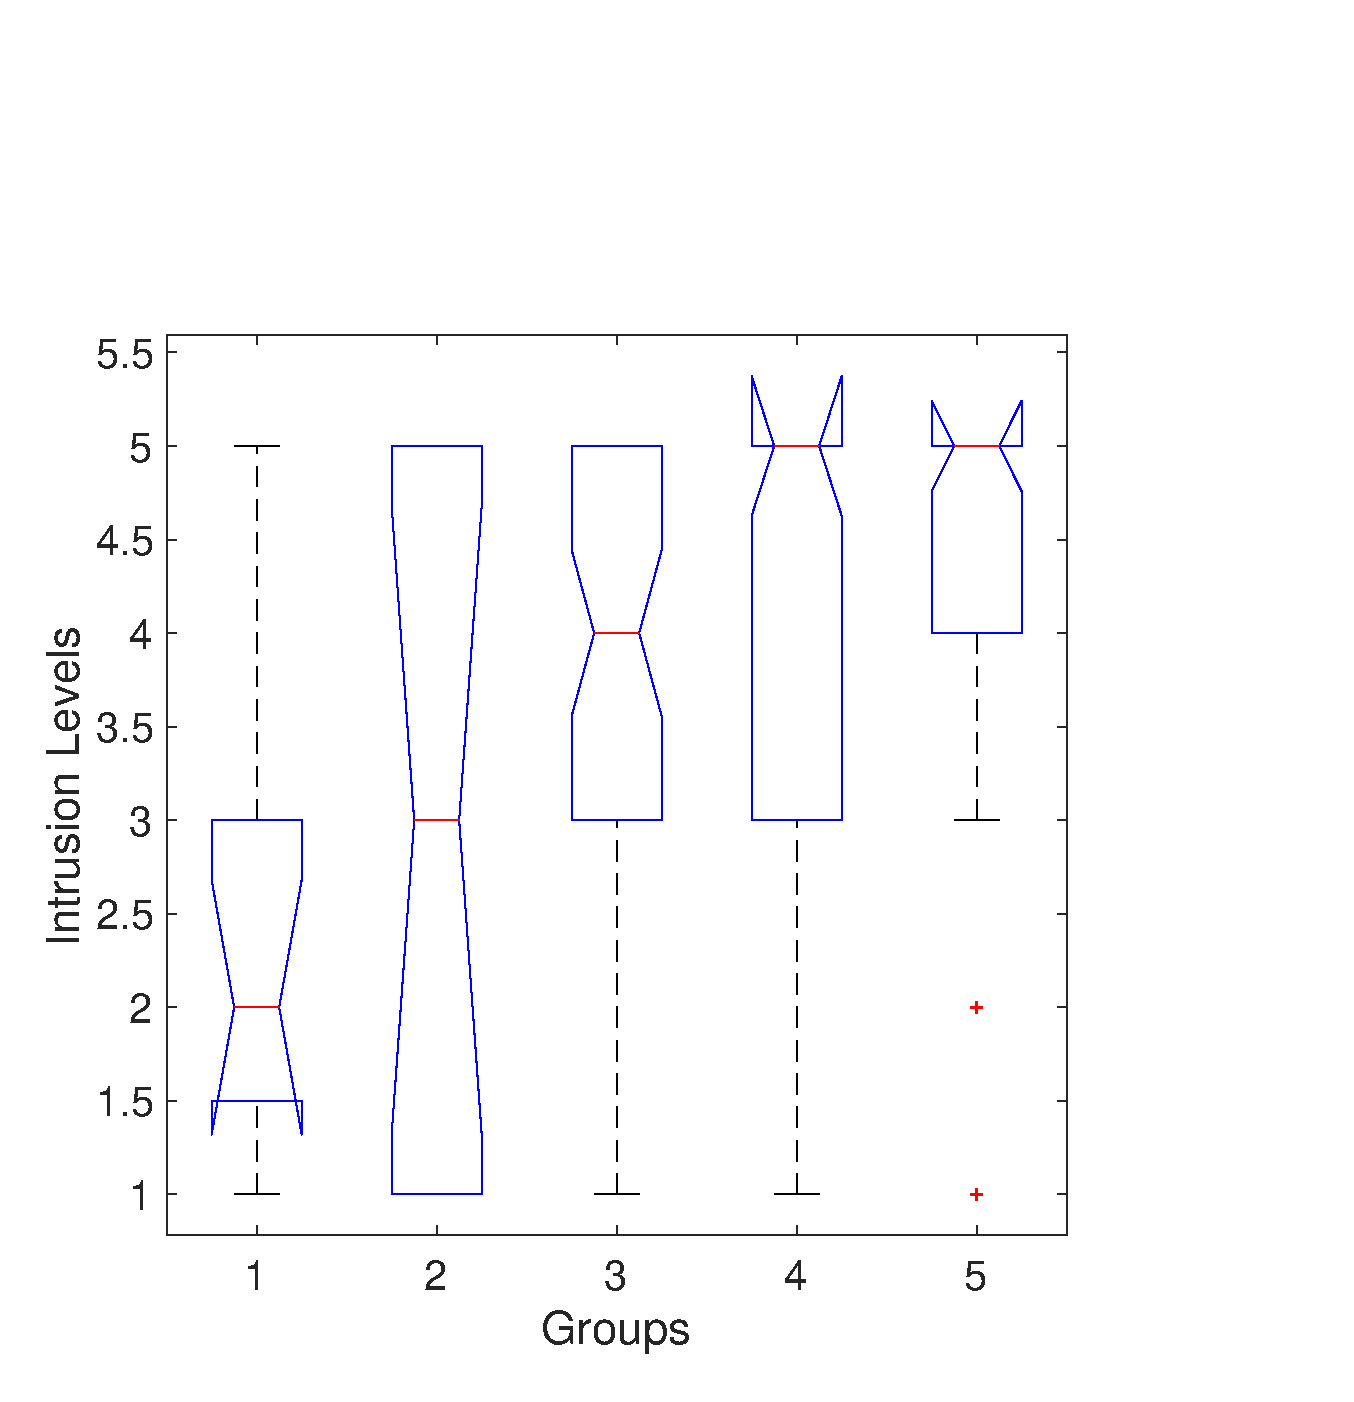
\includegraphics[width=0.45\linewidth]{./images/micro_box}} \newline
\subtop[Camera\label{fig:se_cam}]{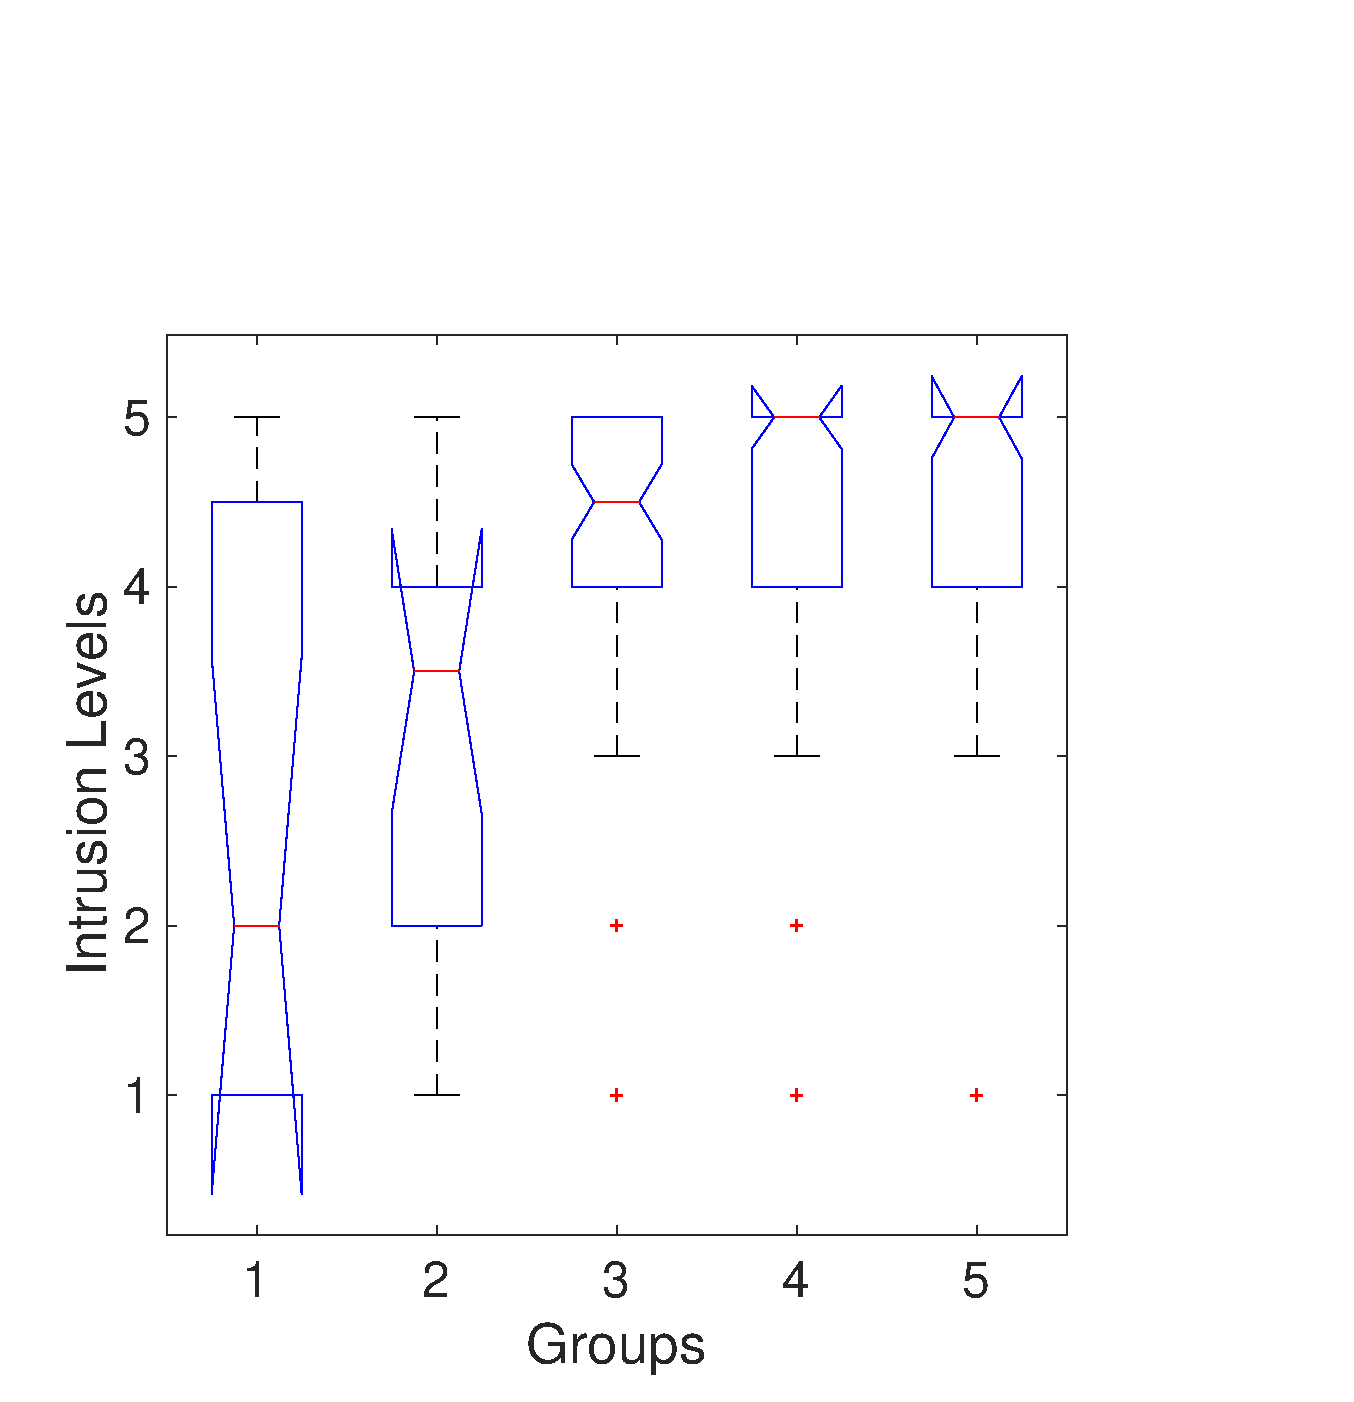
\includegraphics[width=0.45\linewidth]{./images/camera_box}}\hspace{1em}
\subtop[Bluetooth\label{fig:se_blue}]{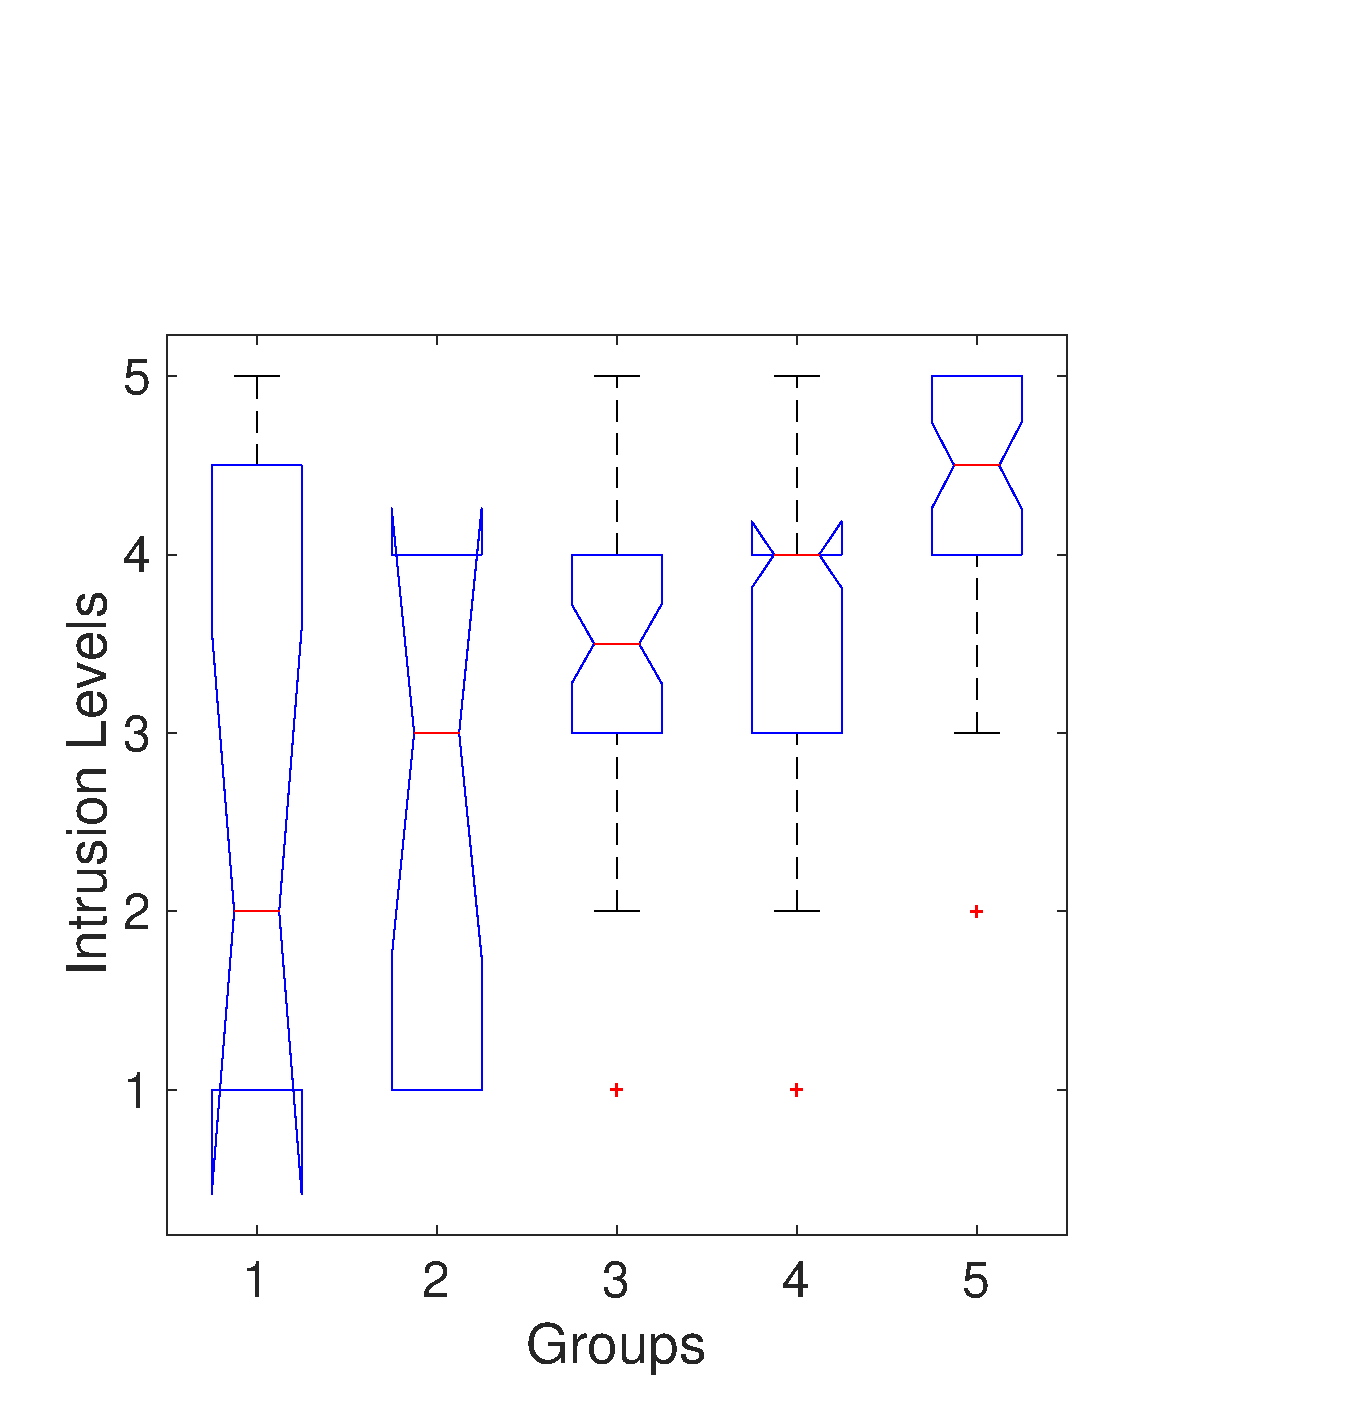
\includegraphics[width=0.45\linewidth]{./images/blue_box}}
\caption{Box Plots Indicating the Population Spread of each Group}
\label{fig:st3}
\end{figure}


\subsubsection{Perception of Individual Stakeholders Grouped on the Intrusion of Stakeholders in General}

In this section, we try to see if the intrusion level perception by people of Stakeholders in general defines the intrusion of the individual stakeholders. In other words we examine the significant differences between groups formed by using question 12's responses (which looks into the perception of users for stakeholders in general) on the perception of
each individual stakeholder. Since there are 5 different responses to question 12 ,this results in five independent groups. The groups 1 to 5 have 7, 11, 32, 69 and 70 people in each group respectively. More detailed information about the employment, education, gender and age distribution in the groups is given in tables \ref{tab:emp_stak}, \ref{tab:edu_stak}, \ref{tab:gender_stak} and \ref{tab:year_stak}. The mean and variances of each group formed is depicted in figures \ref{fig:st1} and \ref{fig:st2}.

\begin{figure}[htp]
\subtop[Mean of each Group for each Stakeholder\label{fig:st1}]{\includegraphics[width=0.5\linewidth,height=0.45\linewidth]{./images/stakeholders_group_meanQ12}}
\subtop[Variance of each Group for each Stakeholder\label{fig:st2}]{\includegraphics[width=0.5\linewidth,height=0.45\linewidth]{./images/stakeholders_group_varianceQ12}}
\caption{Mean and Variance of Groups}
\label{fig:st3}
\end{figure}

To start, we examine all the groups simultaneously for all the individual stakeholders.The Kruskal-Wallis H-test since the data is discrete and not normally distributed. Further detail about the reason the test is chosen is provided in the previous section \ref{result:sensor}. The null hypothesis states that all the groups rate the intrusion of each stakeholder in a similar way. The alternative hypothesis is that the groups rate the intrusion of each stakeholder in a significantly different way.

The resulting p-values of this test are displayed in table \ref{tab:kw_stak}. As it is seen, the test pronounces that all the groups are significantly different at an alpha with 0.05 for all stakeholders. 


\begin{table}[h!]
  \centering
  \caption{Kuskal-Wallis Test for Stakeholders}
  \label{tab:kw_stak}
  \begin{tabular}{cc}
    \toprule
     Stakeholder & p-value \\
    \midrule
    Corporation & 2.1432e-05 \\
    Non-Governmental Organization & 0.0221\\
    Educational Institution & 0.0396\\
    Government & 0.0024\\ 
    \bottomrule
  \end{tabular}
\end{table}

This prompts us to take a closer look at which of the groups are significantly different from each other for each stakeholder. For this, we continue the experiment by performing a Dunn's Test with p-values adjusted by the Bonferroni Method. The results from the tests are shown in table \ref{tab:dunn_stak}. The test was done for all stakeholders since the Kruskal-Wallis test denoted that all groups differ significantly for all stakeholders. 

Looking at the stakeholder corporation, it is seen that groups (1,4), (1,5) and (2,5) differ significantly. This goes to show that groups with larger differences in their outlook to stakeholders as a whole view corporations in a significantly different way. Figure \ref{fig:st_corp} shows the spread of each group for corporations. It is observed that adjacent groups have a large overlap.

For the non-governmental organizations, only the groups (1,5) differ significantly. This goes to show that groups that do not find stakeholders intrusive and groups that find stakeholders very intrusive rate the intrusion of Non-Governmental Organization in significantly different ways. Additionally, it shows that groups with large differences in the perception of stakeholders have significant differences in their perceptions on NGOs. Figure \ref{fig:st_ngo} reinforces this claim.

For Educational Institutions, none of pairwise comparisons have p-values below 0.05. This goes to show that the intrusion of Educational Institutions by all groups does not differ significantly, that is all groups have similar opinions. Figure \ref{fig:st_edu} shows that all groups have significant overlap.

Lastly, for the stakeholder government, the groups (1,4) and (1,5) differ significantly. This goes to show that groups that view the intrusion of stakeholders with a larger difference view Government in a significantly different way. Figure \ref{fig:st_gov} shows the spread of the group's opinions on governments. 

The trend observed above is that there is a significant difference in the outlook of individual stakeholders in between groups with larger differences
in their outlook to stakeholders as a whole, with the exception of Educational Institutions where the alternative hypothesis was rejected because on average, users find it lesser intrusive to a level of 2.94 on a scale of five which is least intrusive compared to the others as shown in \ref{exp}. Hence we can conclude that for generally perceived non intrusive stakeholders, there is a similar opinion across various groups. For the rest, there is a significance difference in opinion between groups with larger differences in their outlook to stakeholders as whole. More incentives should be given out to people for generally high intrusive stakeholders and even more so to users from high intrusion groups (such as 4 and 5) to motivate them to give their data to generally perceived intrusive stakeholders. For the lower intrusion stakeholders, there is lesser need of higher rewards for different groups.

\begin{table}[h!]
  \centering
  \caption{Dunn's Test for Stakeholders}
  \label{tab:dunn_stak}
  \begin{tabular}{ccccccc}
    \toprule
     Groups & Corporation & NGO & Educational Institution & Government \\
    \midrule
    (1,2) & 0.9839 & 0.8042 & 0.9565 & 0.6615 \\
    (1,3) & 0.3282 & 0.2351 & 0.8540 & 0.0986 \\
    (1,4) & 0.0240 & 0.1962 & 0.6867 & 0.0289 \\
    (1,5) & 0.0012 & 0.0243 & 0.1254 & 0.0028 \\
    (2,3) & 0.9467 & 0.9992 & 1.0000 & 0.9958 \\
    (2,4) & 0.2047 & 0.9991 & 1.0000 & 0.9252  \\
    (2,5) & 0.0110 & 0.7192 & 0.8415 & 0.3670  \\
    (3,4) & 0.6893 & 1.0000 & 1.0000 & 0.9999 \\
    (3,5) & 0.0197 & 0.8906 & 0.4112 & 0.5794  \\
    (4,5) & 0.4640 & 0.6027 & 0.3427 & 0.7378 \\
    \bottomrule
  \end{tabular}
\end{table}  

\begin{figure}[htp]
\subtop[Corporations\label{fig:st_corp}]{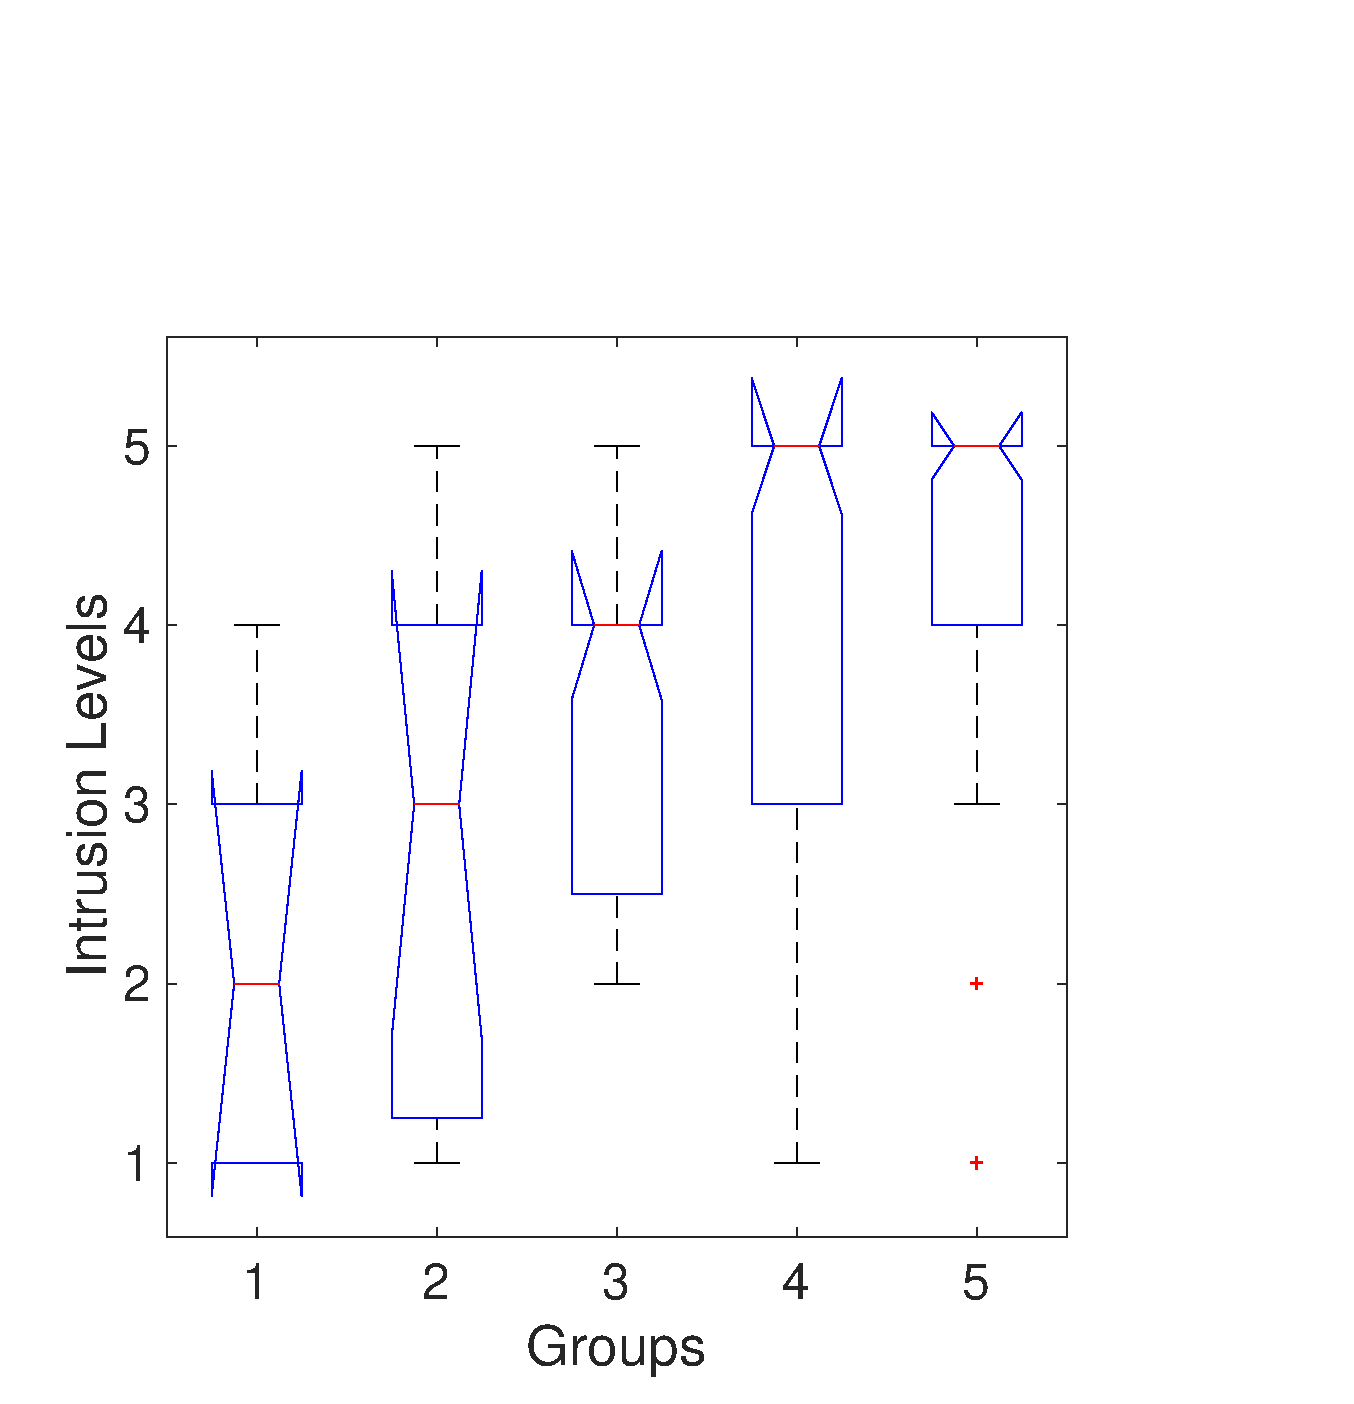
\includegraphics[width=0.4\linewidth]{./images/corp_box}}\hspace{1em}
\subtop[NGO\label{fig:st_ngo}]{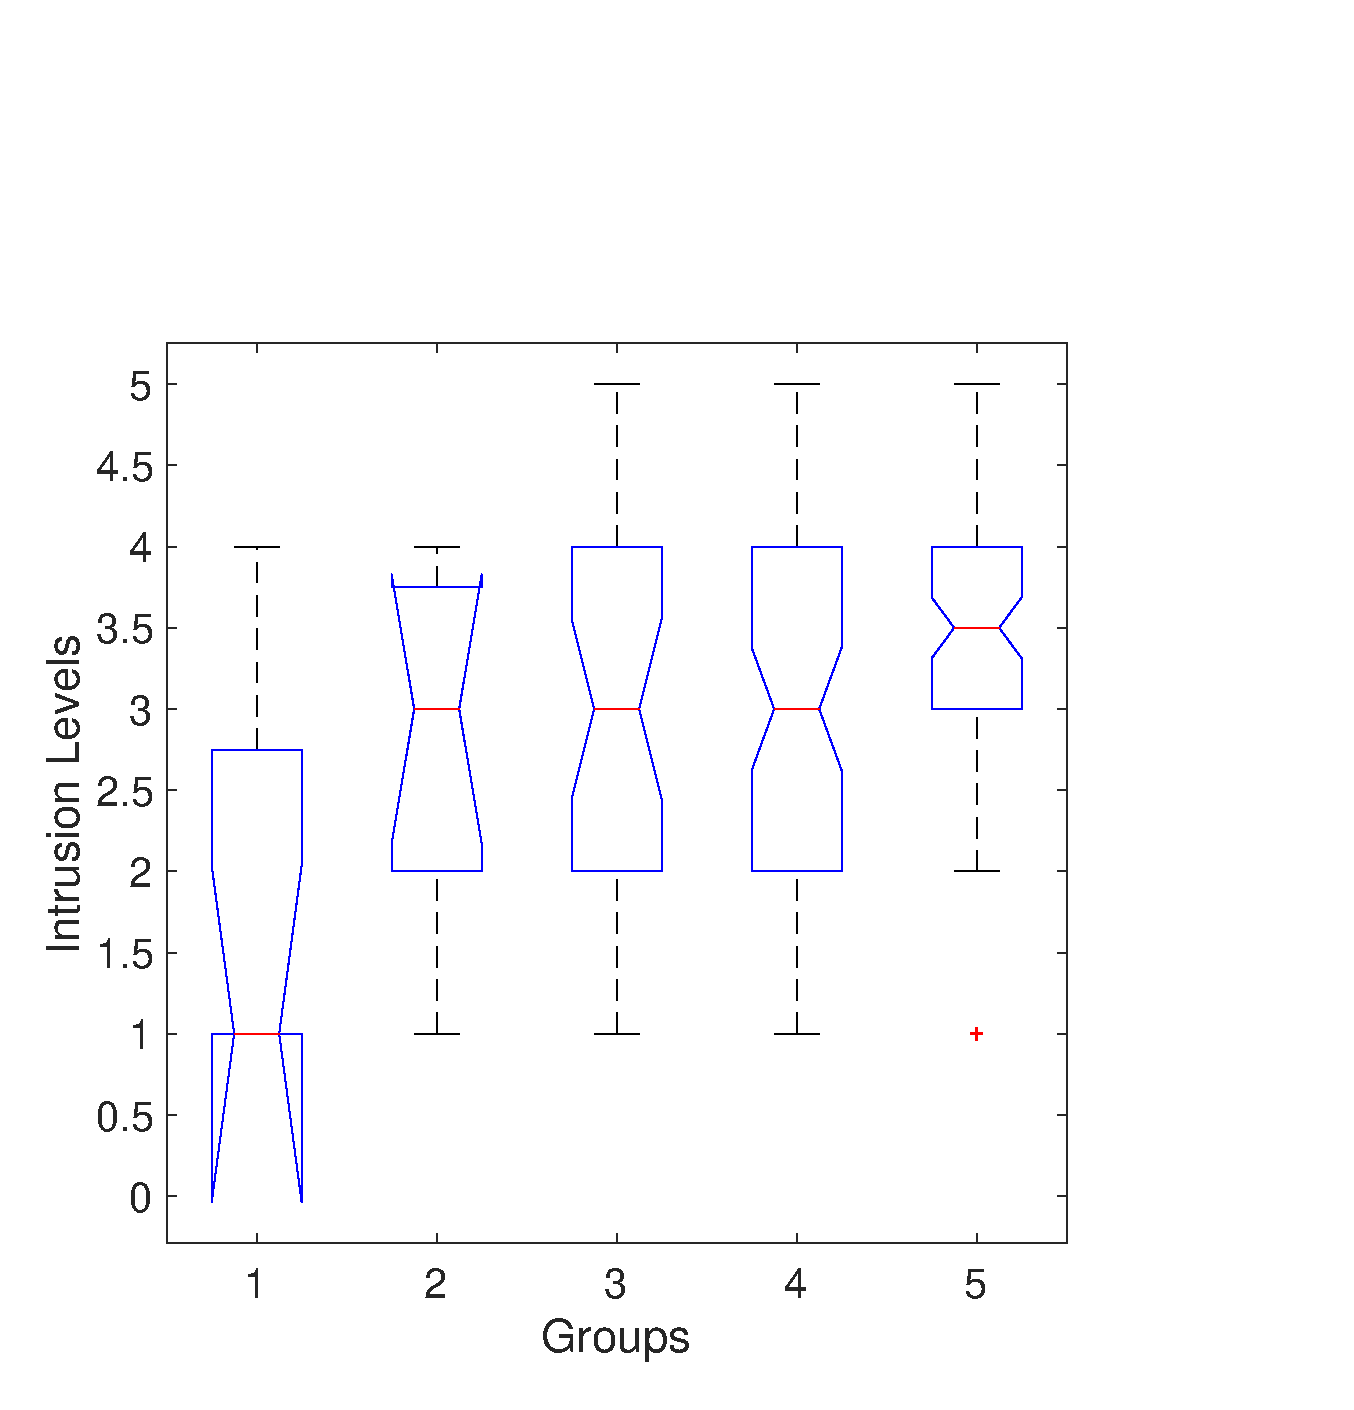
\includegraphics[width=0.4\linewidth]{./images/ngo_box}} \newline
\subtop[Educational Institutions\label{fig:st_edu}]{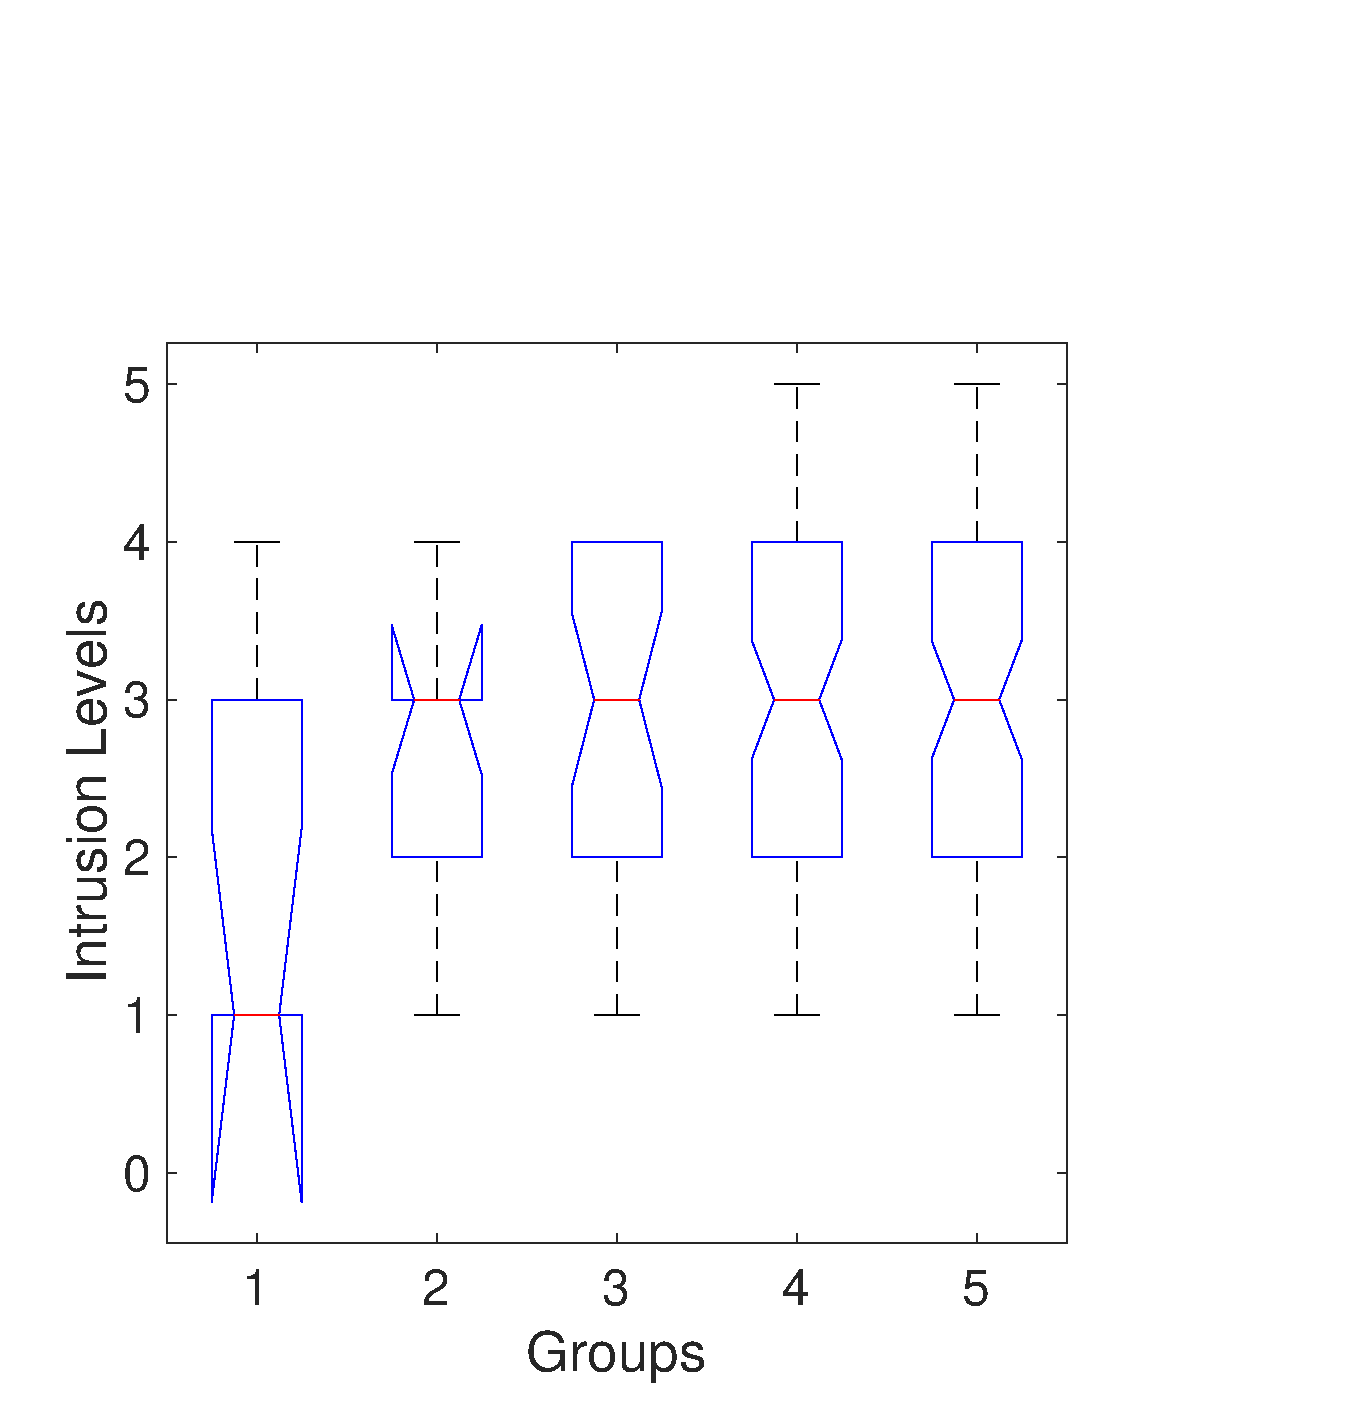
\includegraphics[width=0.4\linewidth]{./images/edu_box}}\hspace{1em}
\subtop[Government\label{fig:st_gov}]{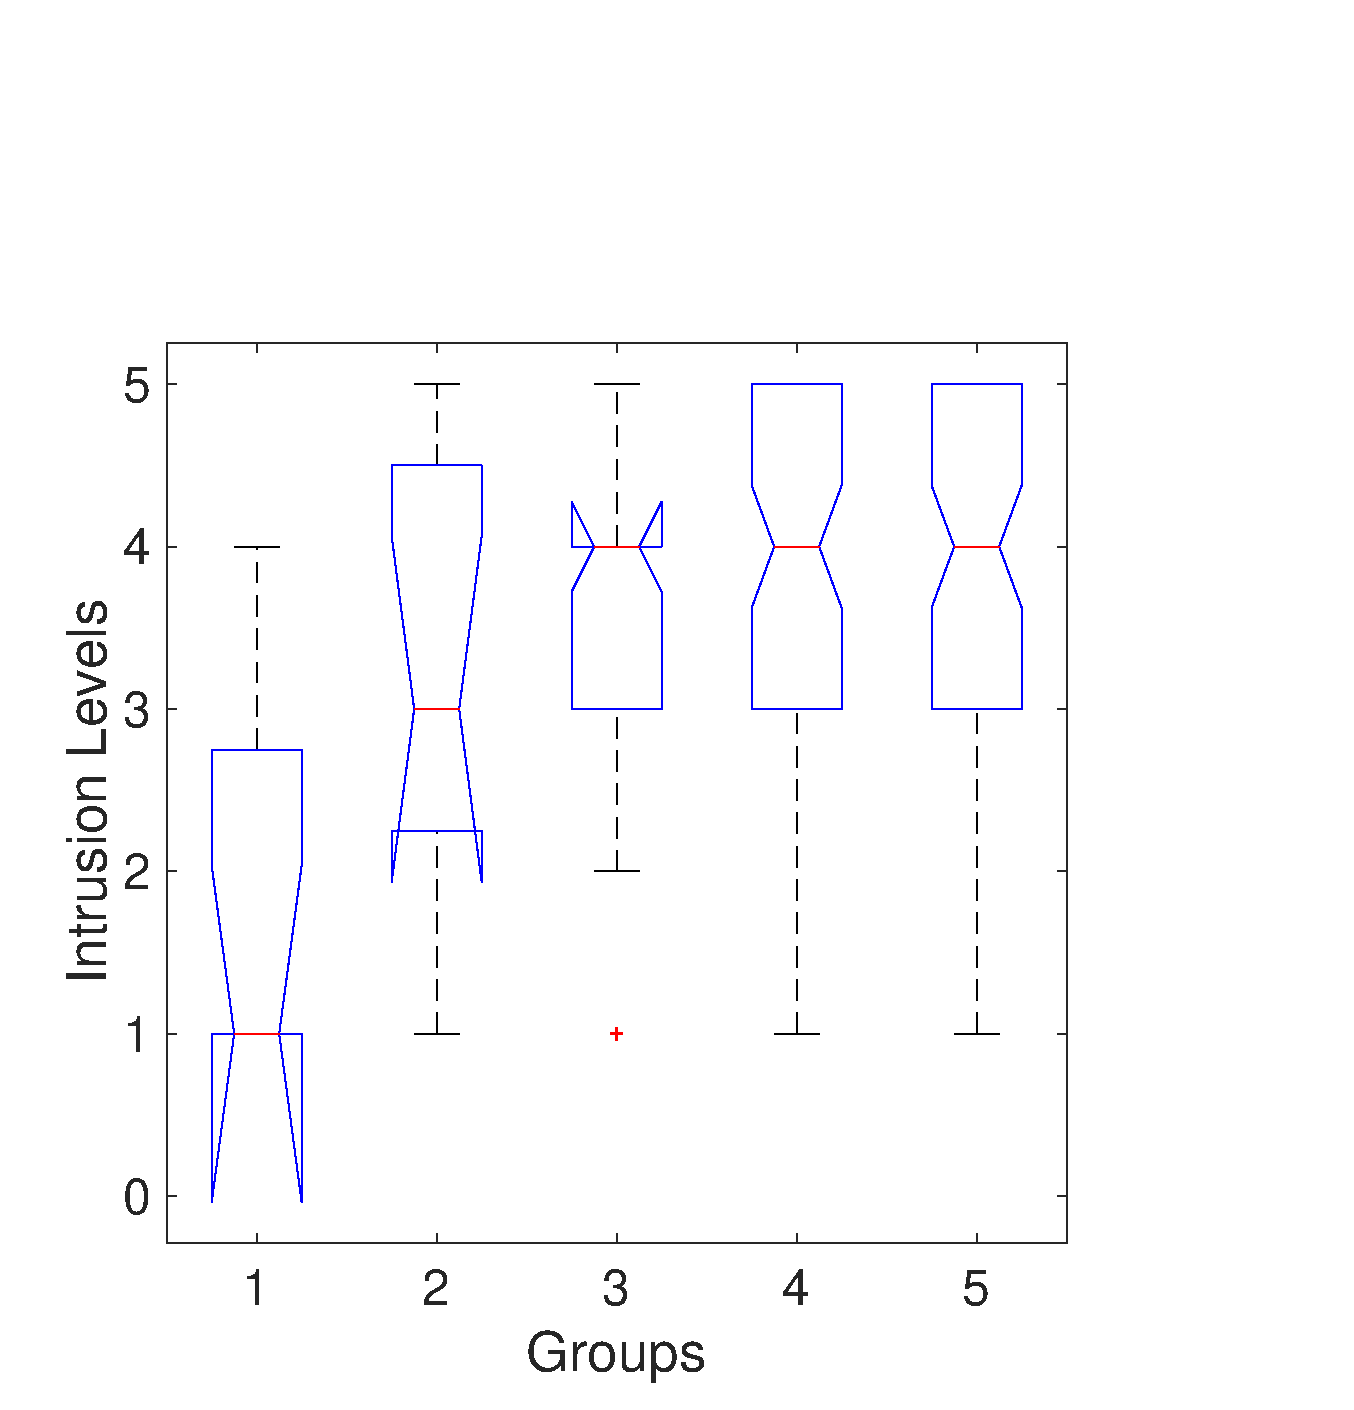
\includegraphics[width=0.4\linewidth]{./images/gov_box}} 
\caption{Box Plots Indicating the Population Spread of each Group}
\label{fig:st3}
\end{figure}

\subsubsection{Perception of Individual Contexts Grouped on the Intrusion of Contexts in General}

In this section, the relationship between the perception of contexts as a whole and the individual contexts is studied. 
To do this, like the above sections the data is partitioned into groups based on the answers given question 14, which asks the user the perception of intrusion of contexts in a data request. There are five groups in total partitioned using the responses given to question 14. Group one to five have each 12, 11, 42, 74 and 50 people respectively. Additional
information about the groups on employment, education , gender and year of birth is given in tables \ref{tab:emp_c}, \ref{tab:edu_c}, \ref{tab:gender_c} and \ref{tab:year_c}. 

Like in the previous sections, since the data is discrete and not normal, we use the Kruskal-Wallis test to compare the groups perceptions on various contexts \ref{result:sensor}. The alpha value is considered to be 0.05. The results of the test are presented in table \ref{tab:kw_c}. As it is seen, the test says that there is a significant difference between all the groups for all contexts.

\begin{figure}[htp]
\subtop[Mean of each Group for each Context\label{fig:co1}]{\includegraphics[width=0.5\linewidth,height=0.45\linewidth]{./images/contexts_group_meanQ14}}
\subtop[Variance of each Group for each Context\label{fig:co2}]{\includegraphics[width=0.5\linewidth,height=0.45\linewidth]{./images/contexts_group_varianceQ14}}
\caption{Mean and Variance of Groups}
\label{fig:co3}
\end{figure}

\begin{table}[h!]
  \centering
  \caption{Kuskal-Wallis Test for Contexts}
  \label{tab:kw_c}
  \begin{tabular}{cc}
    \toprule
     Context & p-value \\
    \midrule
    Education &  6.4694e-04 \\
    Entertainment & 1.0660e-04\\
    Environment & 1.3079e-04\\
    Finance & 0.0021\\ 
    Health & 0.0011\\
    Shopping & 5.4227e-05\\ 
    Social Network &  0.0120\\
    Training & 1.2071e-05\\
    Transportation & 4.9043e-04\\ 
    \bottomrule
  \end{tabular}
\end{table} 

Dunn's Test is performed as a post hoc test for all the contexts to observe the exact group pairs that might be significantly different. The results are presented in tables \ref{tab:dunn_c} and \ref{tab:dunn_c1}. 

For the context education, the groups (2,5) and (3,5) are significantly different from each other. The figure \ref{fig:co_educ} shows the spread of the groups. It is seen that groups with larger difference in opinion about contexts have larger differences in opinion about the context education. The reason why the group 1 was not significantly different from group 5 can be attributed to the fact that the population of the survey might not be a representative sample. Secondly, the number of participants in the survey is limited to 189. Thirdly, due to the previous statement the number of people in group 1 is just 12 and the population sample can be unrepresentative of the actual distribution.

For the context entertainment, further investigation shows that groups (1,5), (2,5) and (3,5) are significantly different in each others responses. The figure \ref{fig:co_ent} shows the spread of the groups. Therefore, we infer that groups with higher differences in opinions about contexts (such as groups 1 and 5) have varying opinions of intrusion on entertainment.

For the context environment, groups (2,5) and (3,5) are significantly different from each other. The figure \ref{fig:co_env} shows the spread of the groups. We can come to a similar conclusion to context education as to why group 1 is not significantly different from group 5.

For the context finance, the groups (1,5), and (2,5) are significantly different from each other. The figure \ref{fig:co_finance} shows the spread of the groups and we can infer that groups with bigger differences in opinions on contexts also have significant differences in their opinions on finance context.

In the context health, except for groups (1,5) all the other groups are not significantly different from each other. The figure \ref{fig:co_health} shows the spread of the groups and we can infer people who find contexts non intrusive and very intrusive have significant difference in viewpoint of the health context. As seen, all the other groups have significant overlap with groups 1 and 5.

For the context shopping and social network, none of the groups are significantly different from each other as seen in \ref{fig:co_shopping}. This show that irrespective of their viewpoint about contexts, all groups have similar opinions with the context shopping and social network.

In the context training, the groups (1,5),(3,5) and (4,5) are significantly different from each other. The figure \ref{fig:co_training} shows the spread of the groups. This show that all groups have similar opinions about training contexts except for group 5. The reason for group 2 not being different from group 5 is due to the small population size of group 2. Additionally, more points are mentioned for context education.

Finally for the context transportation, the groups (1,5), (2,5) and (3,5) are significantly different from each other. It is seen in figure \ref{fig:co_nav} that groups 1,2,3 are significantly different form group 5. Group 4 is not significantly different from group 5 due to the fact that the users of group 4 and 5 have closer opinions of contexts than the rest. Hence users who find contexts intrusive will have a significant difference in opinion with sufficiently different groups.

This goes to show that groups that perceive contexts in a more different light tend to have different ways of viewing the individual contexts. We do observe that in some cases (2,5) are significantly different, but (1,5) is not. This can be easily attributed to the low number of responses
and the noise in the data. 

For contexts, we do not make generalizations about the incentives for individual contexts based on the general perception of contexts. Shopping and social networking are considered highly intrusive with values 3.75 and 3.50 and every group had similar opinions. Finance and health are also very intrusive with levels 3.85 and 3.60 on a scale of five. Here a significant difference in opinions was observed between groups with largely different opinions about contexts in general (such as group 1 and 5).

Education and environment are considered 2.83 and 2.92 intrusive on a scale of five, which are the lowest. For these two we observe that there is a significant difference between groups 2 with 5 and 3 with 5. For entertainment and transportation which have medium intrusion levels of 3.39 and 3.38 on a scale of five and it is observed that groups 1, 2, 3 differ significantly from group 5. It is still observed that groups with higher intrusion perception of contexts (such as group 5) view some contexts in a more intrusive light and should be incentivized more for those.

\begin{table}[h!]
  \centering
  \caption{Dunn's Test for Contexts Part 1}
  \label{tab:dunn_c}
  \begin{tabular}{cccccccc}
    \toprule
     Groups & Education & Entertainment & Environment & Finance & Health  \\
    \midrule
    (1,2)&0.99796&0.99982&0.97055&1.0000&0.63908\\
(1,3)&1.0000&0.99174&1&0.32963&0.076147\\
(1,4)&0.94148&0.19262&0.86998&0.22077&0.042547\\
(1,5)&0.11471&0.0056283&0.21553&0.015364&0.00051115\\
(2,3)&0.9342&1&0.96665&0.31604&0.9999\\
(2,4)&0.32744&0.76121&0.083389&0.21508&0.99963\\
(2,5)&0.0082212&0.082023&0.0048936&0.016365&0.50246\\
(3,4)&0.83617&0.23034&0.10875&1.0000&1.0000\\
(3,5)&0.0064191&0.00086418&0.0012905&0.65747&0.32713\\
(4,5)&0.13825&0.28231&0.60016&0.57519&0.21258\\
    \bottomrule
  \end{tabular}
\end{table}

\begin{table}[h!]
  \centering
  \caption{Dunn's Test for Contexts Part 2}
  \label{tab:dunn_c1}
  \begin{tabular}{ccccccc}
    \toprule
     Groups & Shopping & Social Network & Training & Transportation  \\
    \midrule
(1,2) &1.0000&0.99831&1.0000&1.0000\\
(1,3)&0.99992&0.94767&1.0000&0.9722\\
(1,4)&0.18309&0.089135&0.90197&0.23809\\
(1,5)&0.015842&0.10636&0.010906&0.016376\\
(2,3)&1.0000&1.0000&1&0.98253\\
(2,4)&0.39426&0.70552&0.99778&0.30509\\
(2,5)&0.052334&0.7272&0.068368&0.026144\\
(3,4)&0.038351&0.21259&0.58123&0.51397\\
(3,5)&0.00050454&0.29374&2.1697e-05&0.012924\\
(4,5)&0.69535&1.0000&0.0033189&0.55629\\
  \end{tabular}
\end{table} 


\begin{figure}[htp]

\subtop[Education\label{fig:co_educ}]{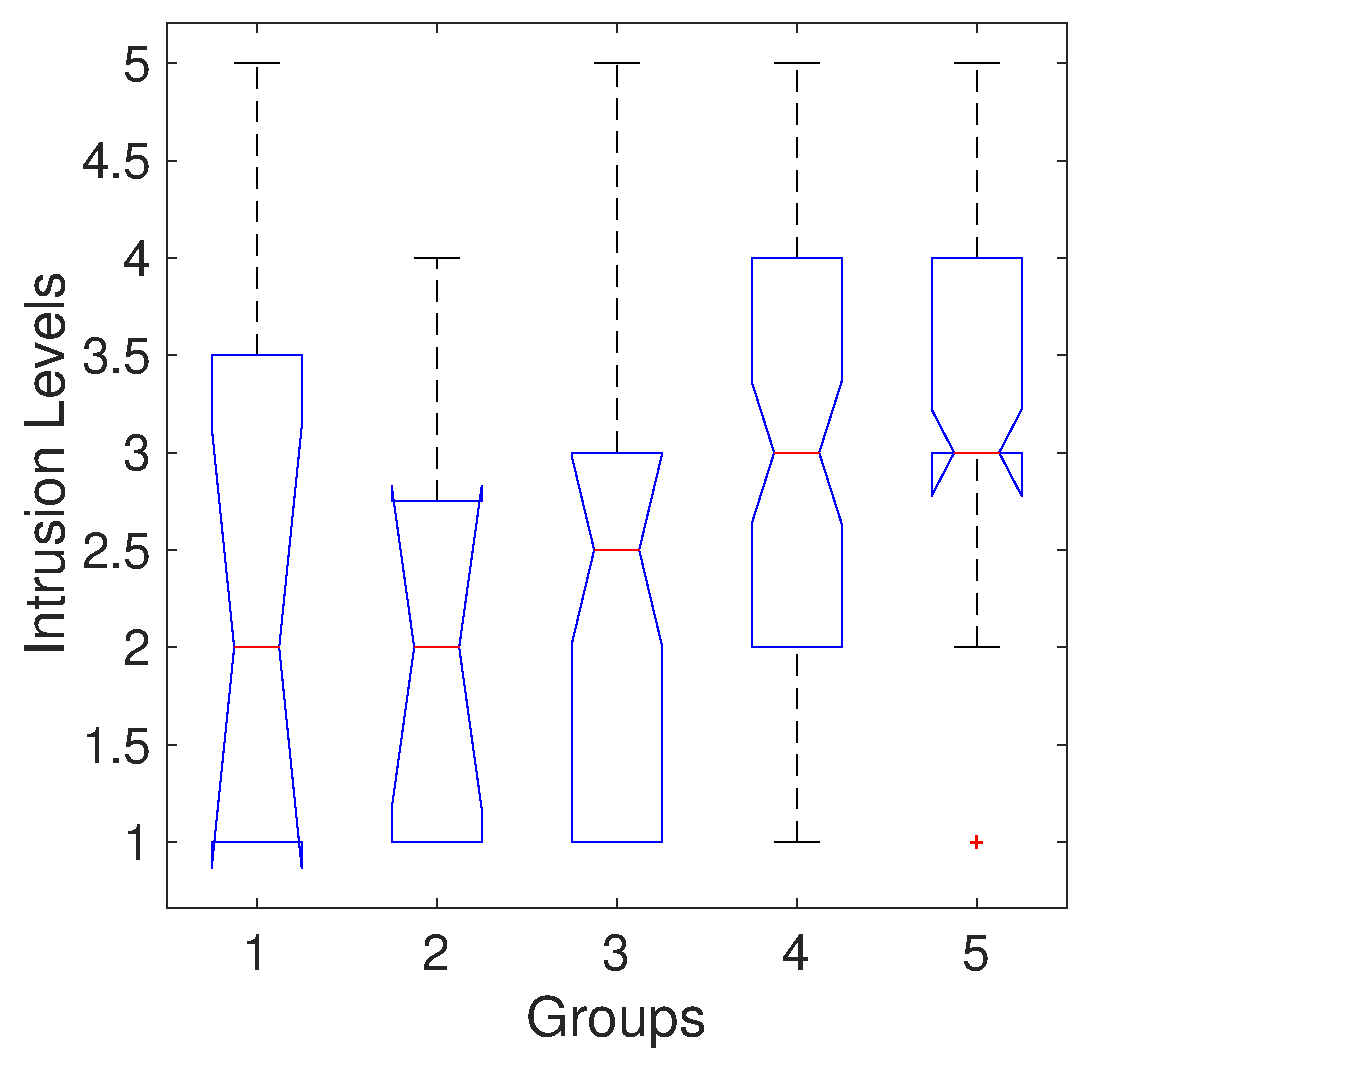
\includegraphics[width=0.4\linewidth]{./images/educ_box}}\hspace{1em}
\subtop[Entertainment\label{fig:co_ent}]{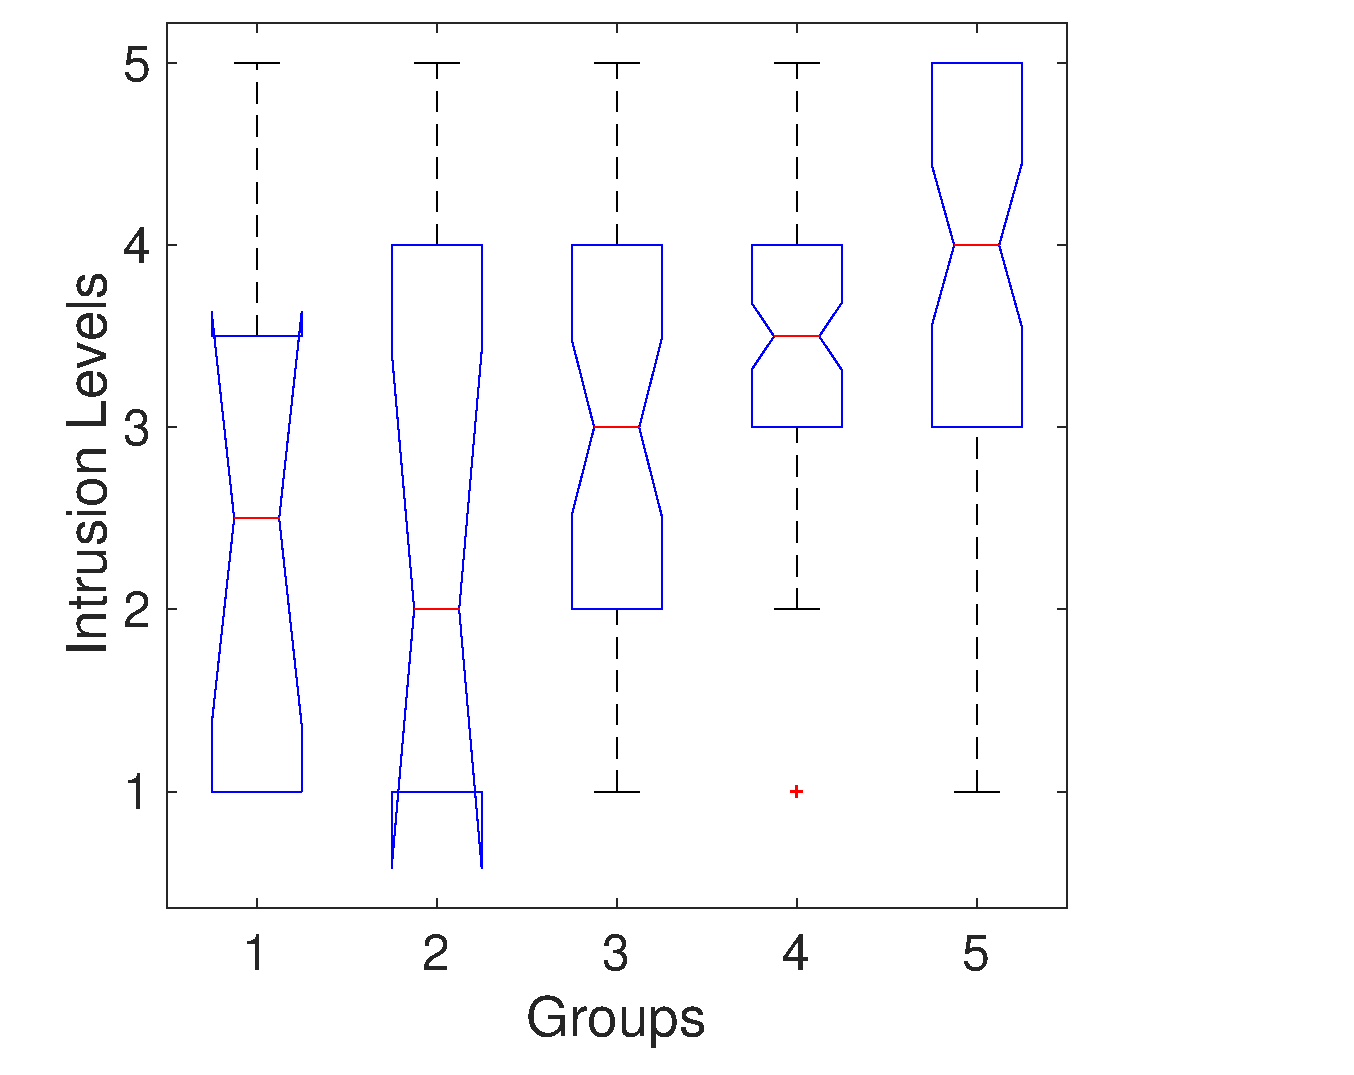
\includegraphics[width=0.4\linewidth]{./images/ent_box}} \newline
\subtop[Environment\label{fig:co_env}]{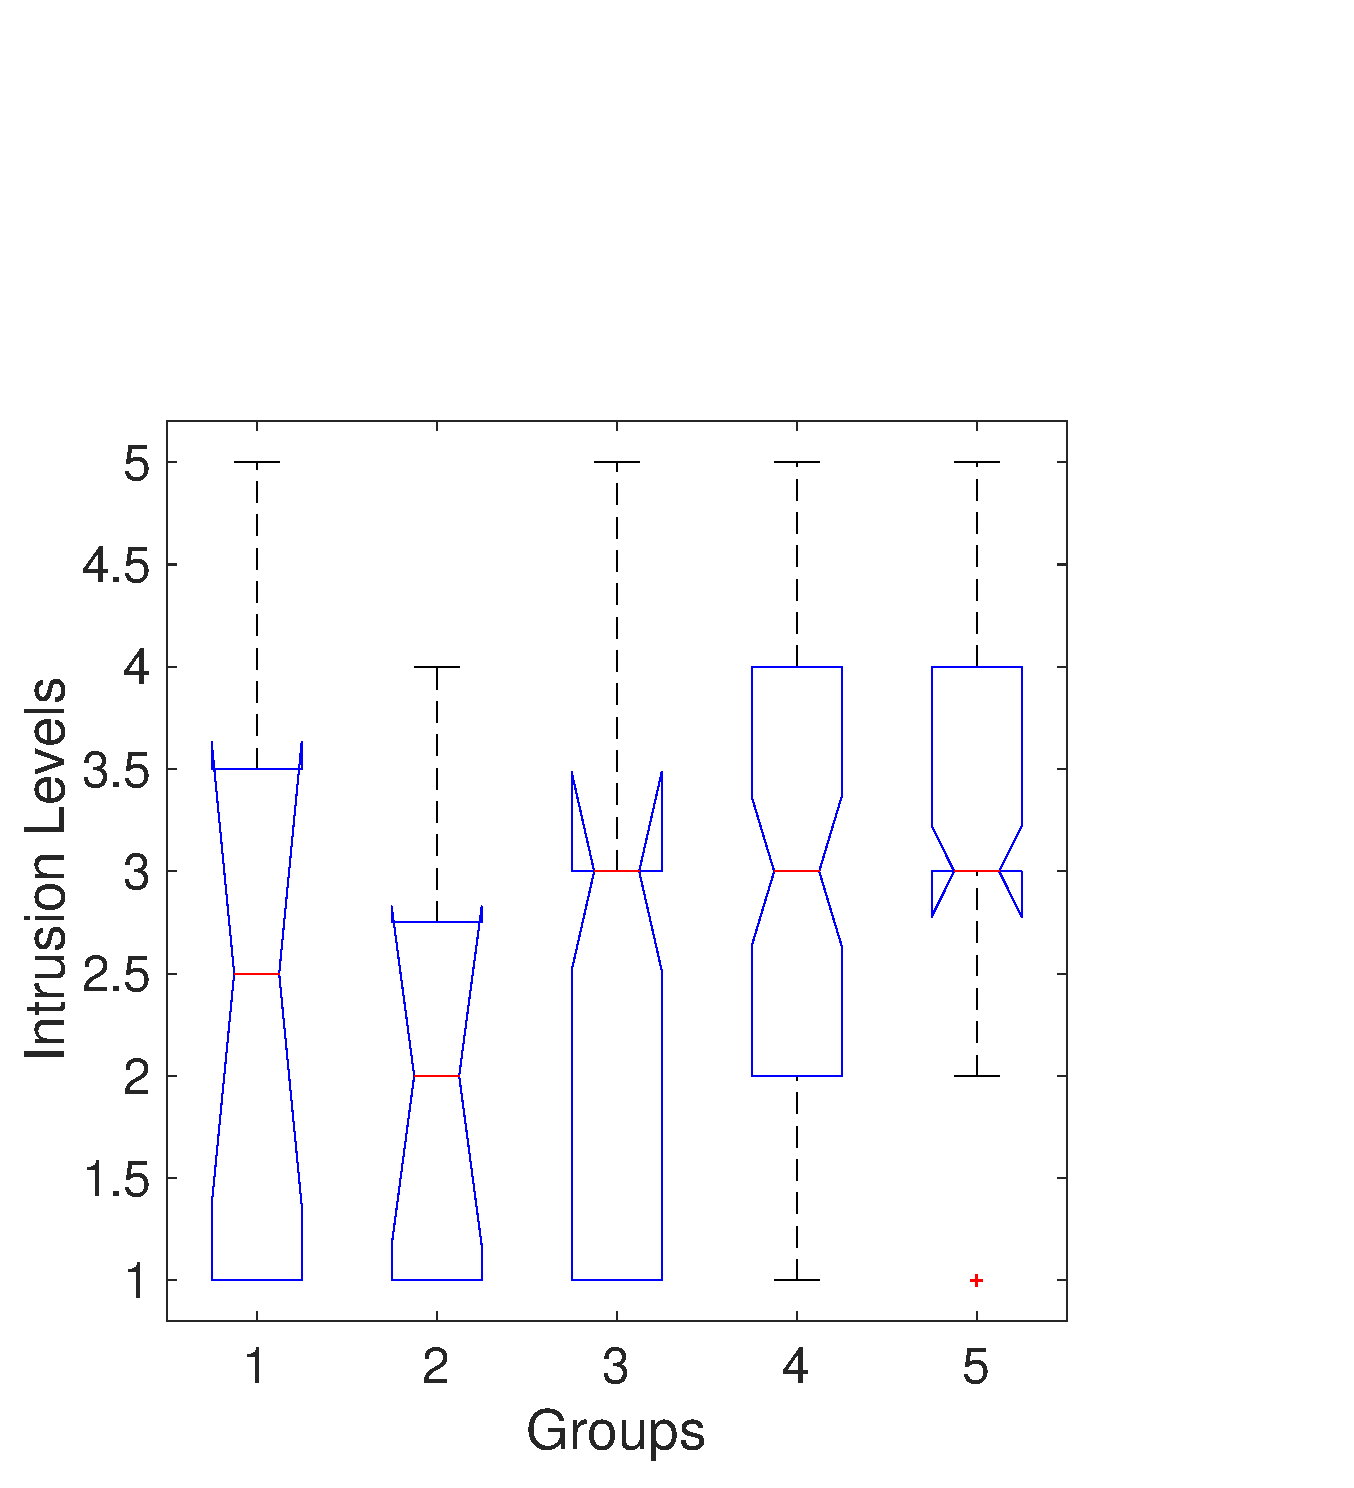
\includegraphics[width=0.4\linewidth]{./images/env_box}}\hspace{1em}
\subtop[Finance\label{fig:co_finance}]{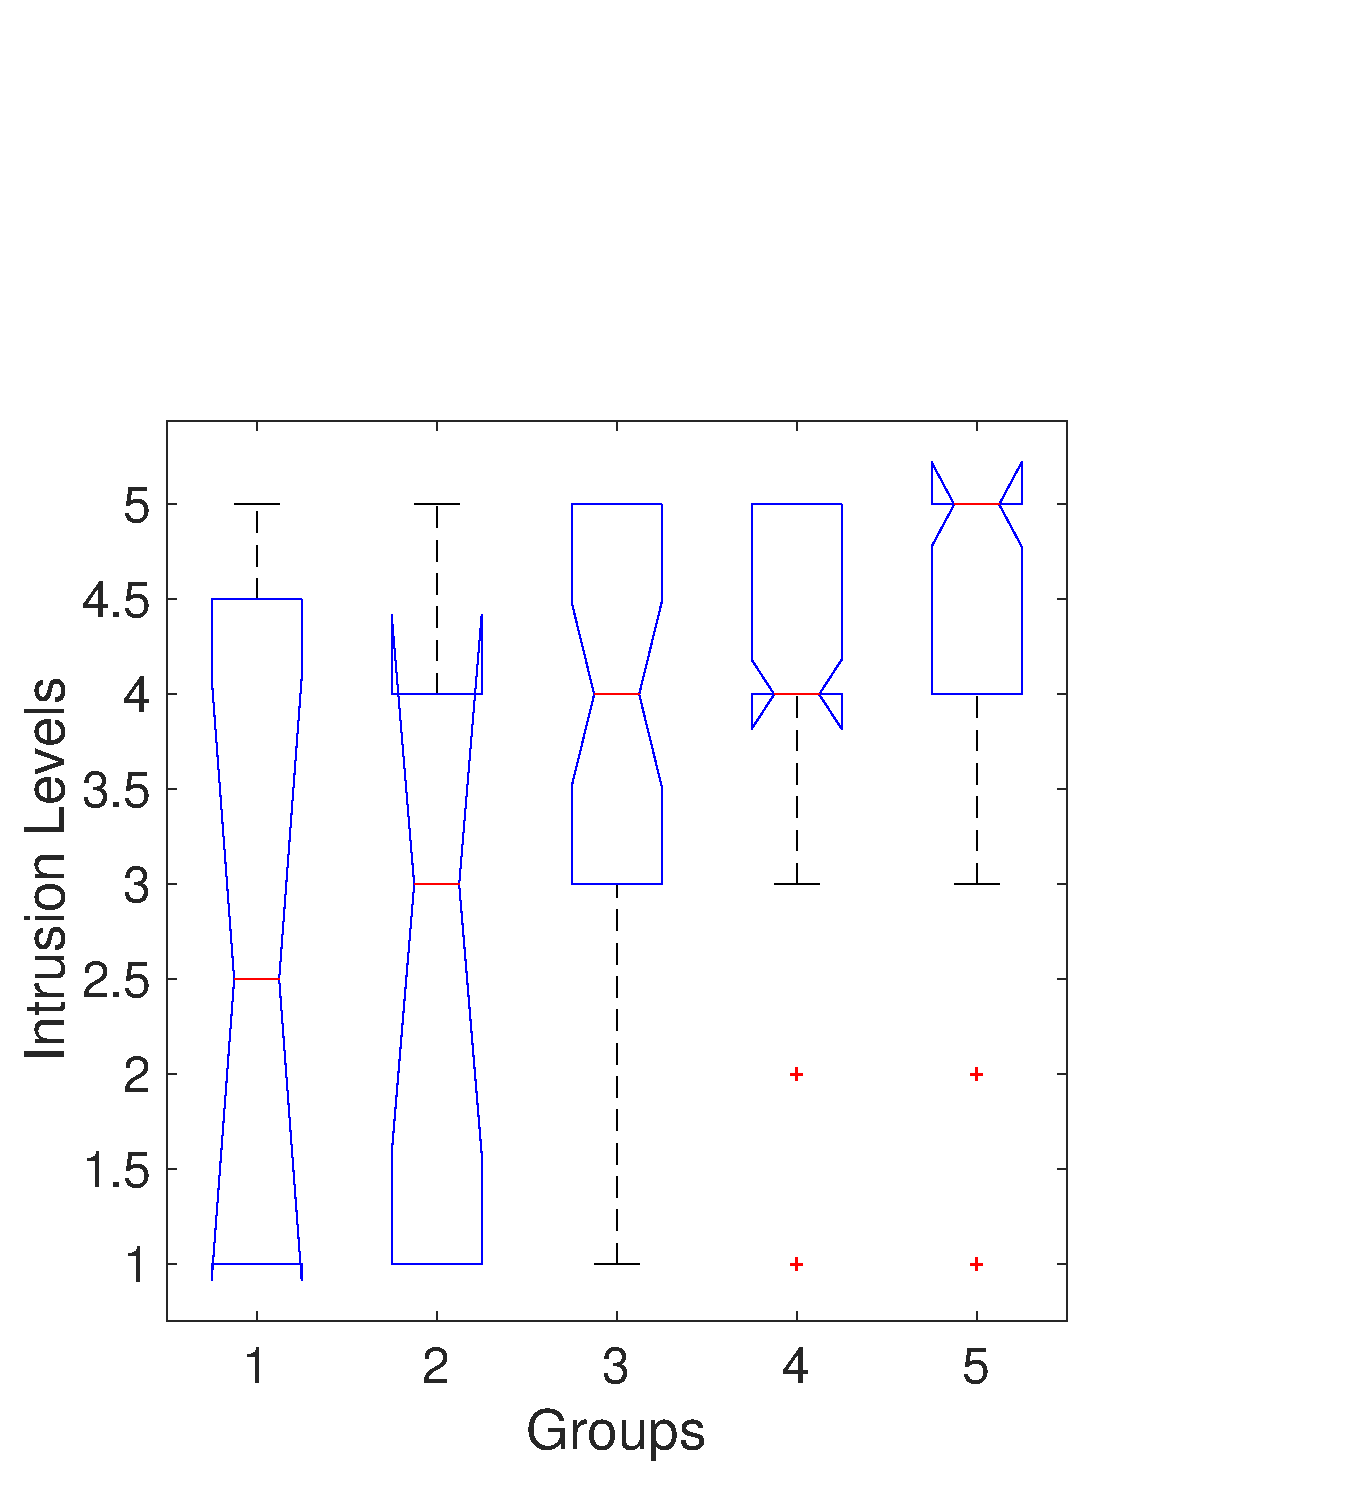
\includegraphics[width=0.4\linewidth]{./images/finance_box}} \newline
\subtop[Health\label{fig:co_health}]{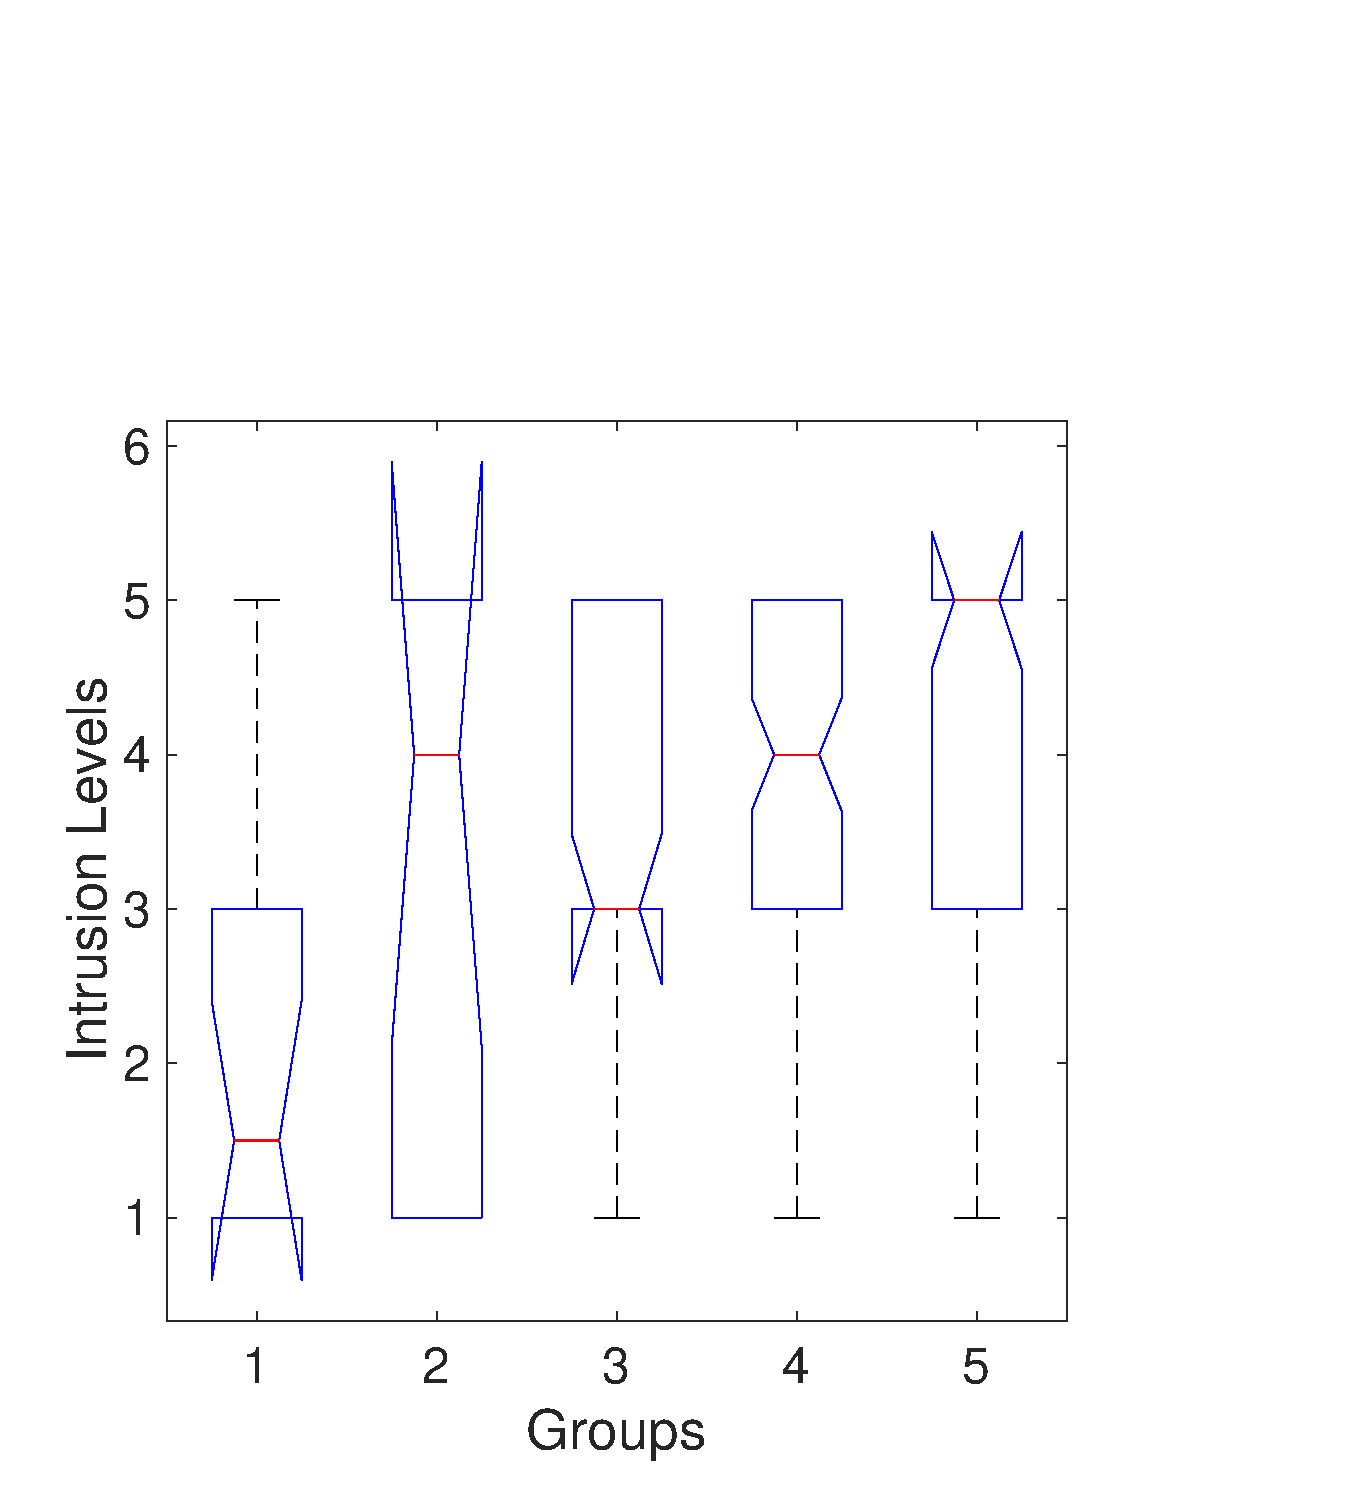
\includegraphics[width=0.4\linewidth]{./images/health_box}}\hspace{1em}
\subtop[Shopping\label{fig:co_shopping}]{\includegraphics[width=0.4\linewidth]{./images/shopping_box}} 
\caption{Mean and Variance of Groups}
\label{fig:st3}
\end{figure}

\begin{figure}[htp]
\subtop[Social Networking\label{fig:co_social}]{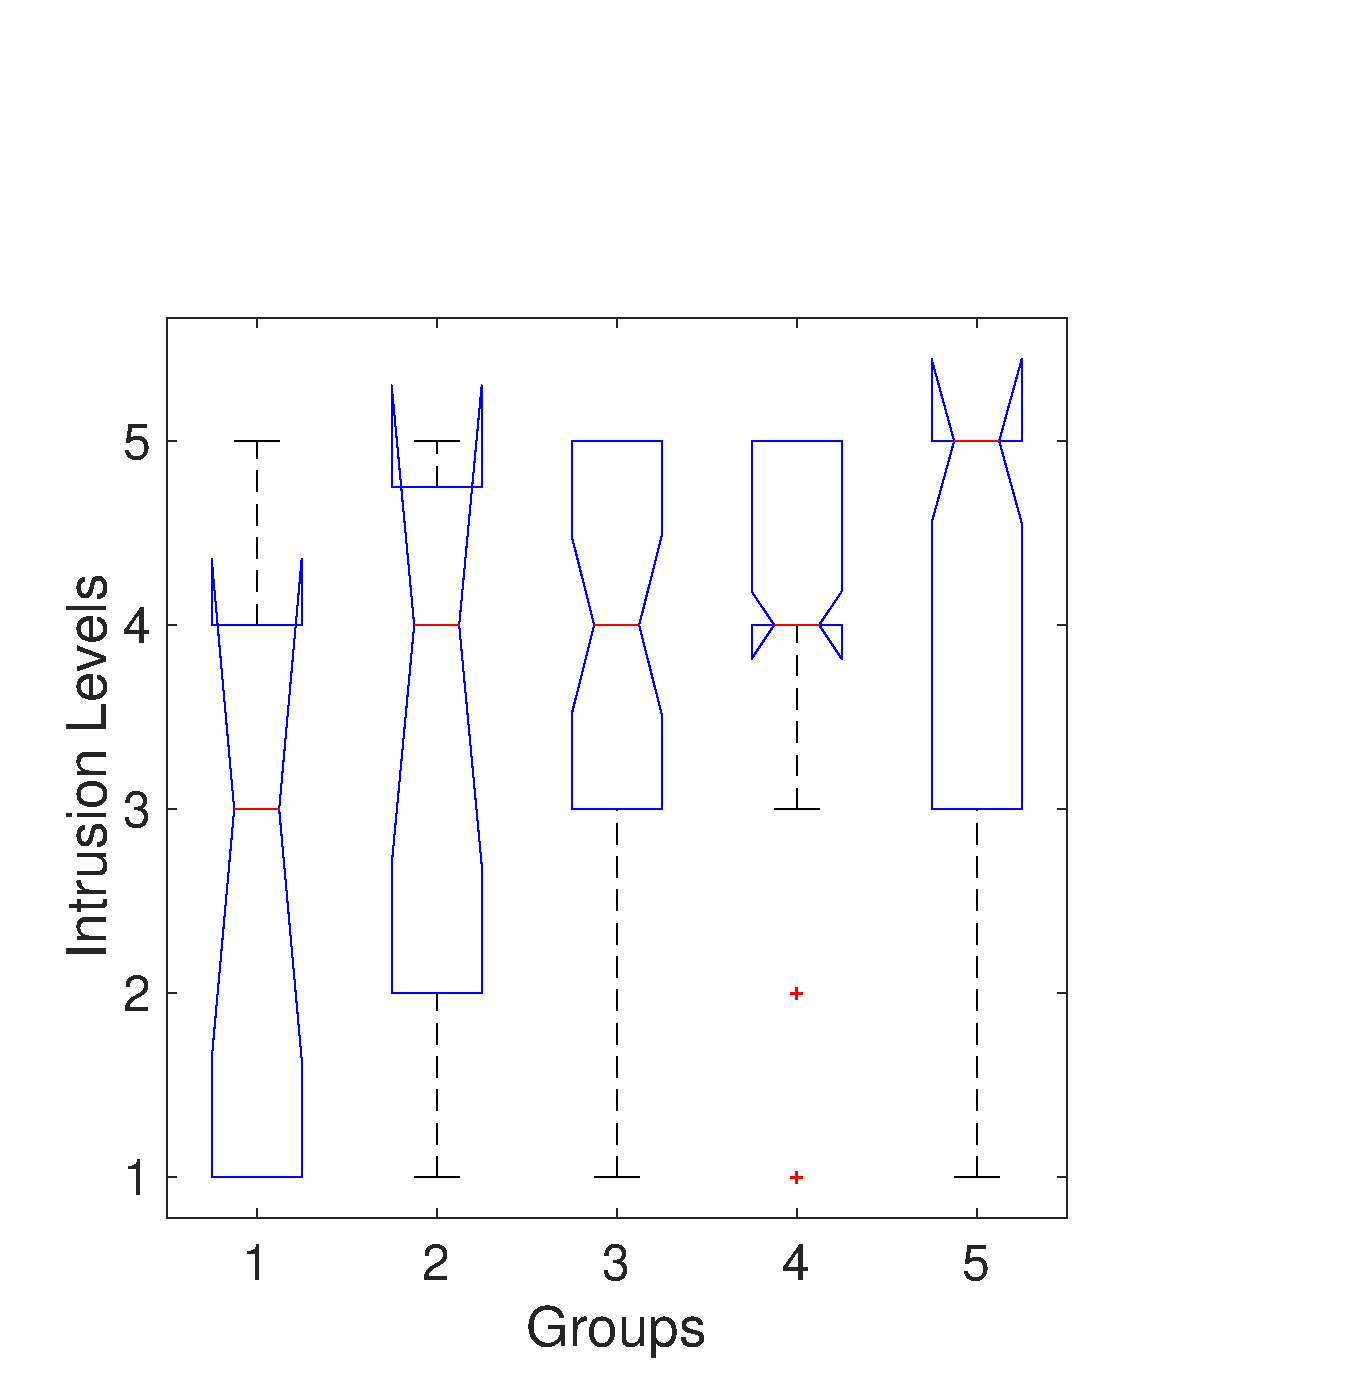
\includegraphics[width=0.4\linewidth]{./images/social_box}}\hspace{1em}
\subtop[Training\label{fig:co_training}]{\includegraphics[width=0.4\linewidth]{./images/training_box}}\newline
\centering
\subtop[Navigation\label{fig:co_nav}]{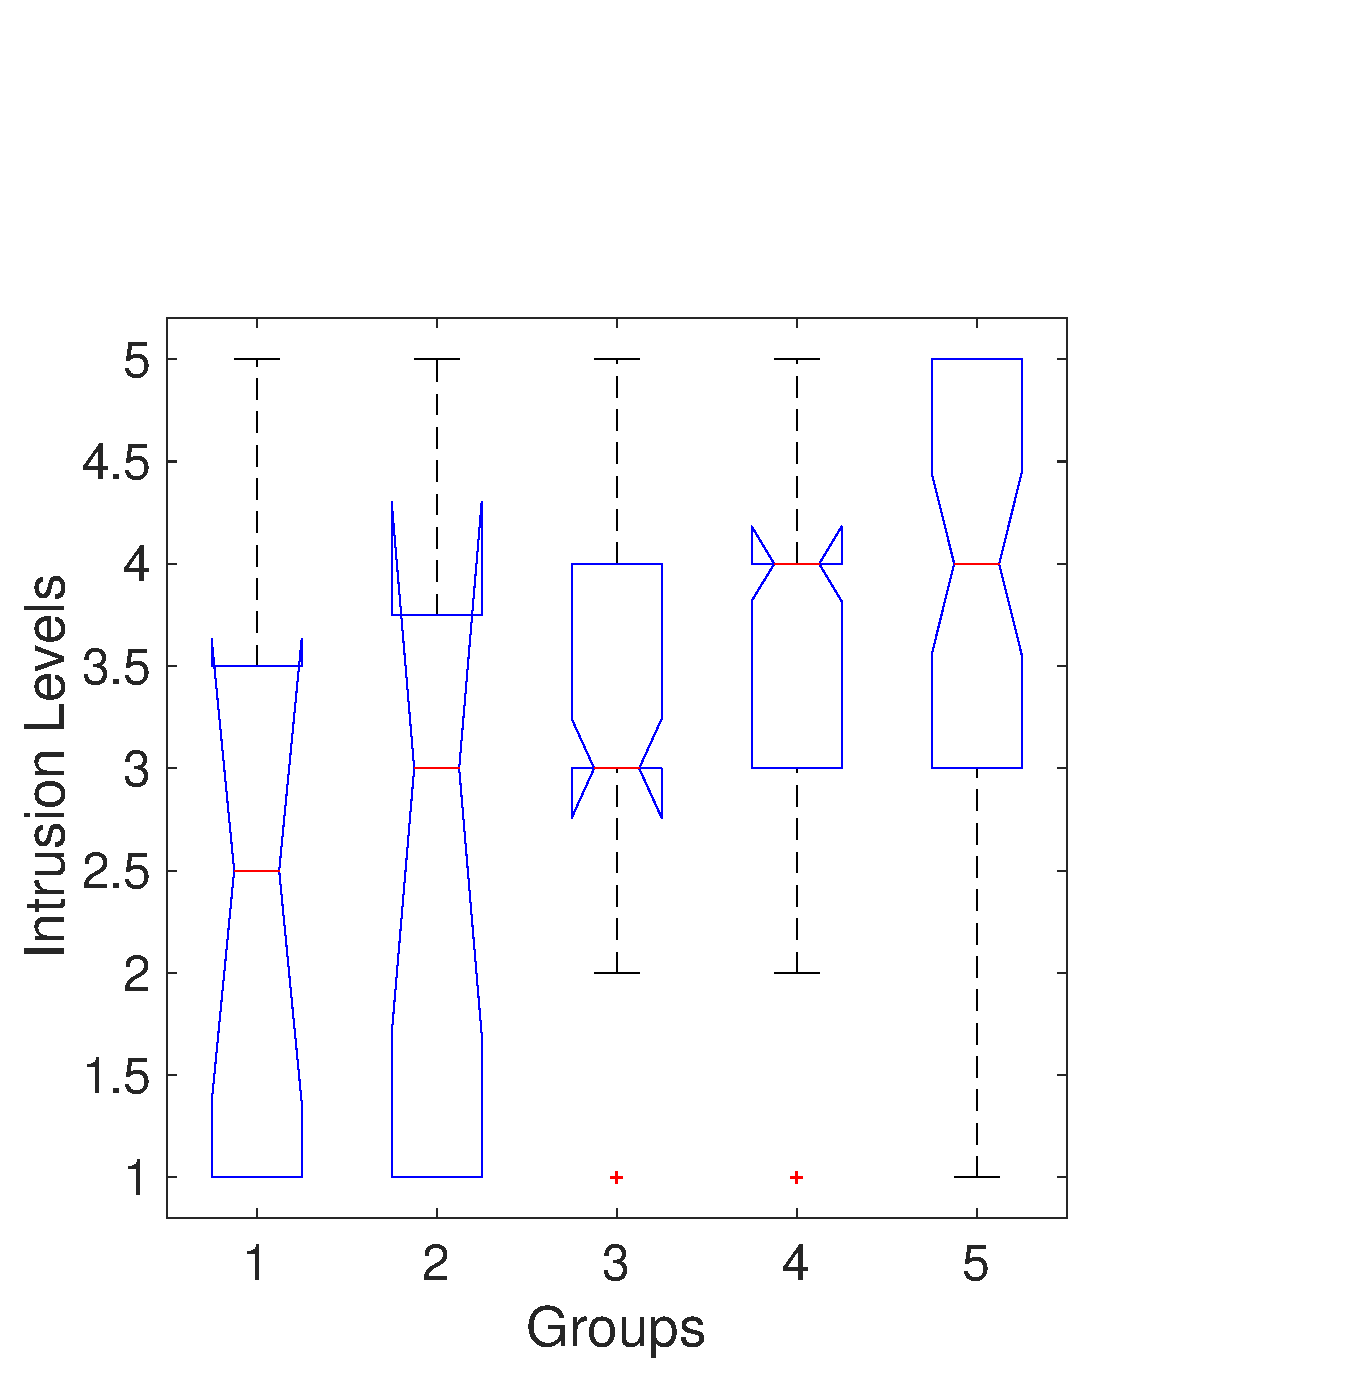
\includegraphics[width=0.4\linewidth]{./images/nav_box}}
\caption{Mean and Variance of Groups}
\label{fig:st3}
\end{figure}

Above, the various intrusion and their relationship with their sub-features was examined. If there was a constant relationship between both, categorization of sub-features in the experiment would be redundant. The above shows that categorizations of sub-features is still essential to the computational model since the data above is not sufficient to make claims about the relationship. In the future, deploying this survey with a larger more representative population can help reduce the number of categorization questions in the model and perhaps even eliminate the categorizations all together.

\section{Findings from the Experiment Data}

The social experiment described in chapter \ref{exp} took place using 10 participants. Out of the total 3 days of the experiment, 3 of the participants did not answer data requests on day 2 and 3. The mobile application ran successfully on all participants phones even after being switched off. All data was successfully recorded on the server. Participants were not paid but were asked to behave like they were paid, so results might skew from the ideal scenario. A trial was run to see if the application created works and to get user feedback on the usability. Additionally, using the data collected on the server, the relationship between data sharing and incentives is examined. 

\begin{figure}[htp]
\subtop[Actual improvements in Credit and Privacy\label{fig:actual_pri}]{\includegraphics[width=0.5\linewidth]{./images/heatmap_all_days_privacyimprovement}}\hspace{1em}
\subtop[Improve Privacy and Credit Button\label{fig:button_pri}]{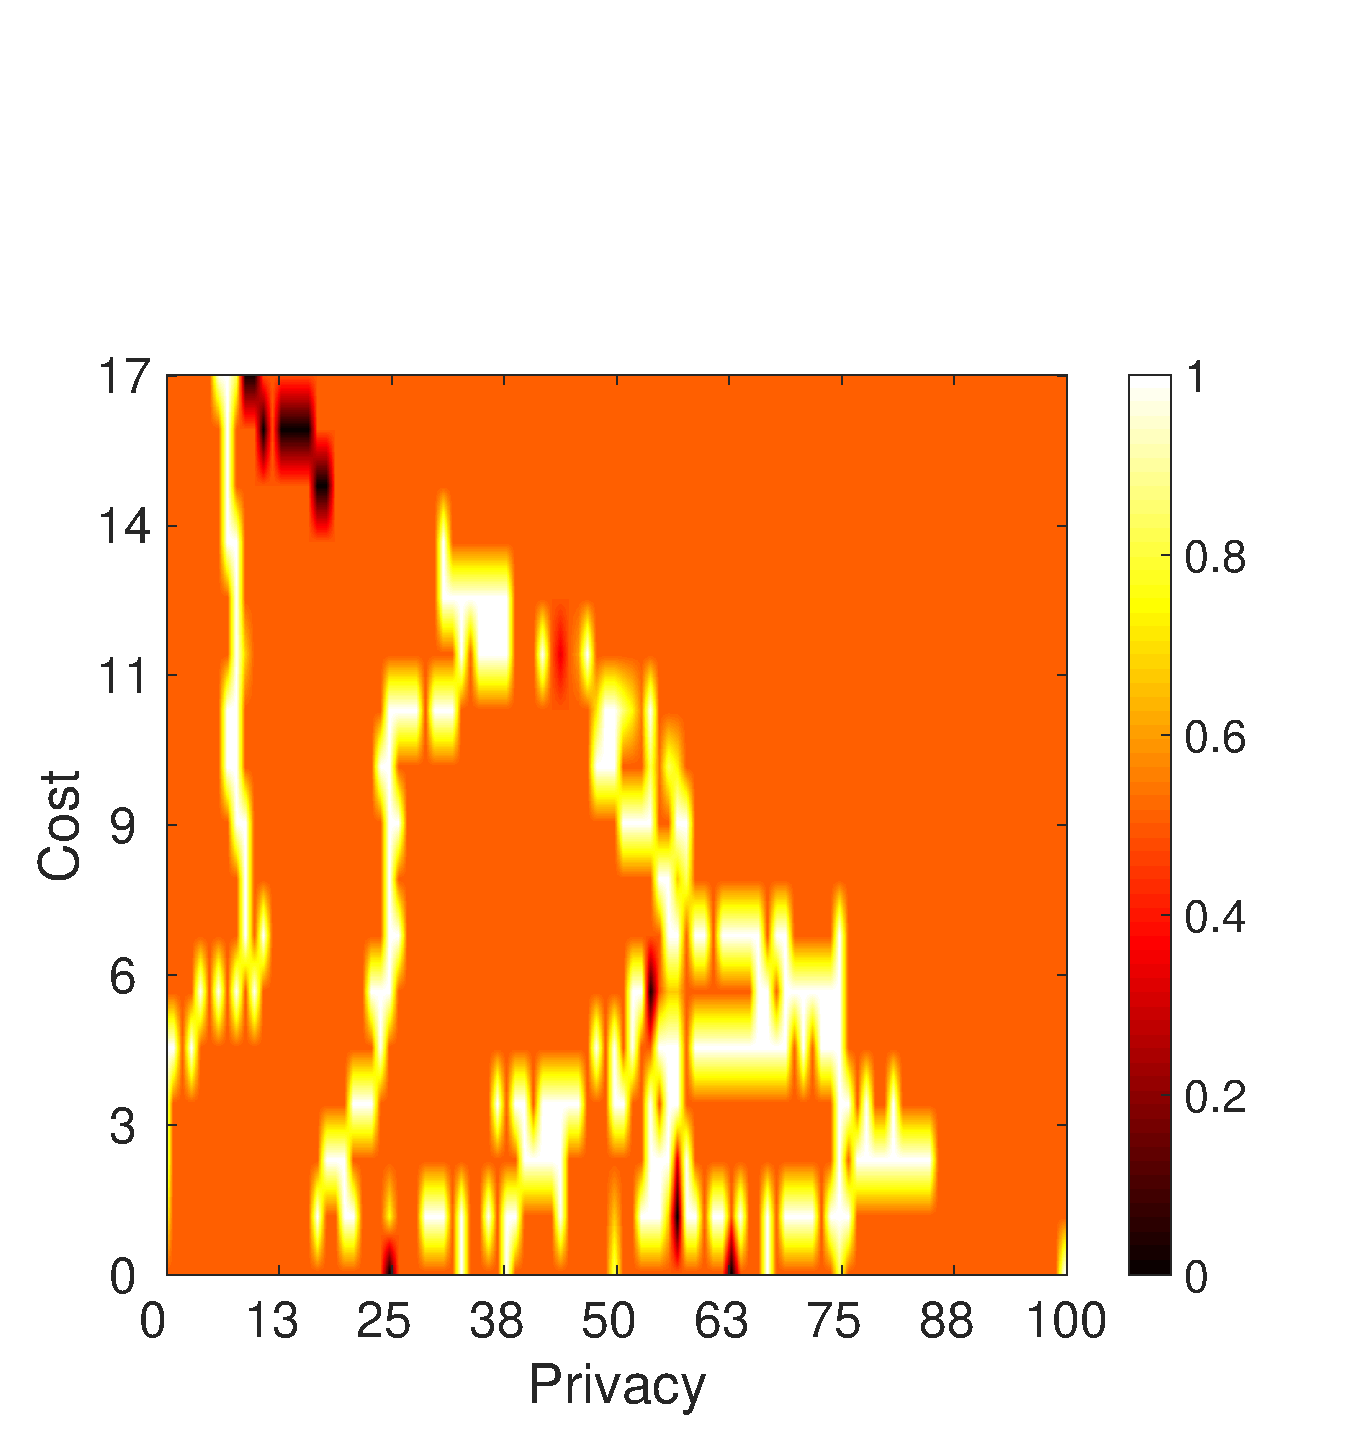
\includegraphics[width=0.5\linewidth]{./images/heatmap_all_days_button}}
\caption{Table Schemas}
\label{fig:st3}
\end{figure}

Figure \ref{fig:button_pri} depicts for every possible cost and privacy the probability of whether users clicked on the privacy button or credit button. The darker color indicates high probability for clicking on the privacy button (0), a light yellow indicates a higher probability for for clicking on the credit button (1) and the orange depicts the probability of clicking on both buttons equally (0.5). It is observed that probability of users to click on the improve privacy button is very close to when they have no privacy at all and a very high cost. This shows that users are more interested to improve their cost than the privacy metric. 

Similarly, figure \ref{fig:actual_pri} depicts for every possible cost and privacy the probability of whether users actually improved their privacy or their credit rather than just wanting to. The darker color indicates high probability for improvement in privacy (0), a light yellow indicates a higher probability for improvement in credit (1) and the orange depicts the probability of an equal improvement in both metrics (0.5). It is observed that the probability of users incrementing their credit is much higher than their privacy just like in the last figure. Users are interested in improving their privacy when they have sufficient cost
and their privacy is becoming lower.

Figures \ref{fig:button_pri} and \ref{fig:actual_pri} are now compared. As observed in \ref{fig:button_pri}, users click on the privacy button close to when they have almost no privacy but it is also observed that they improve their privacy even after clicking on the improve credit button as seen in \ref{fig:actual_pri}. This can be attributed to the fact that users were not comfortable giving data for the data requests that appeared, even tough the intentions were to obtain more credit. This means that they were not incentivized enough for those data requests.


\begin{figure}[ht!]
\centering
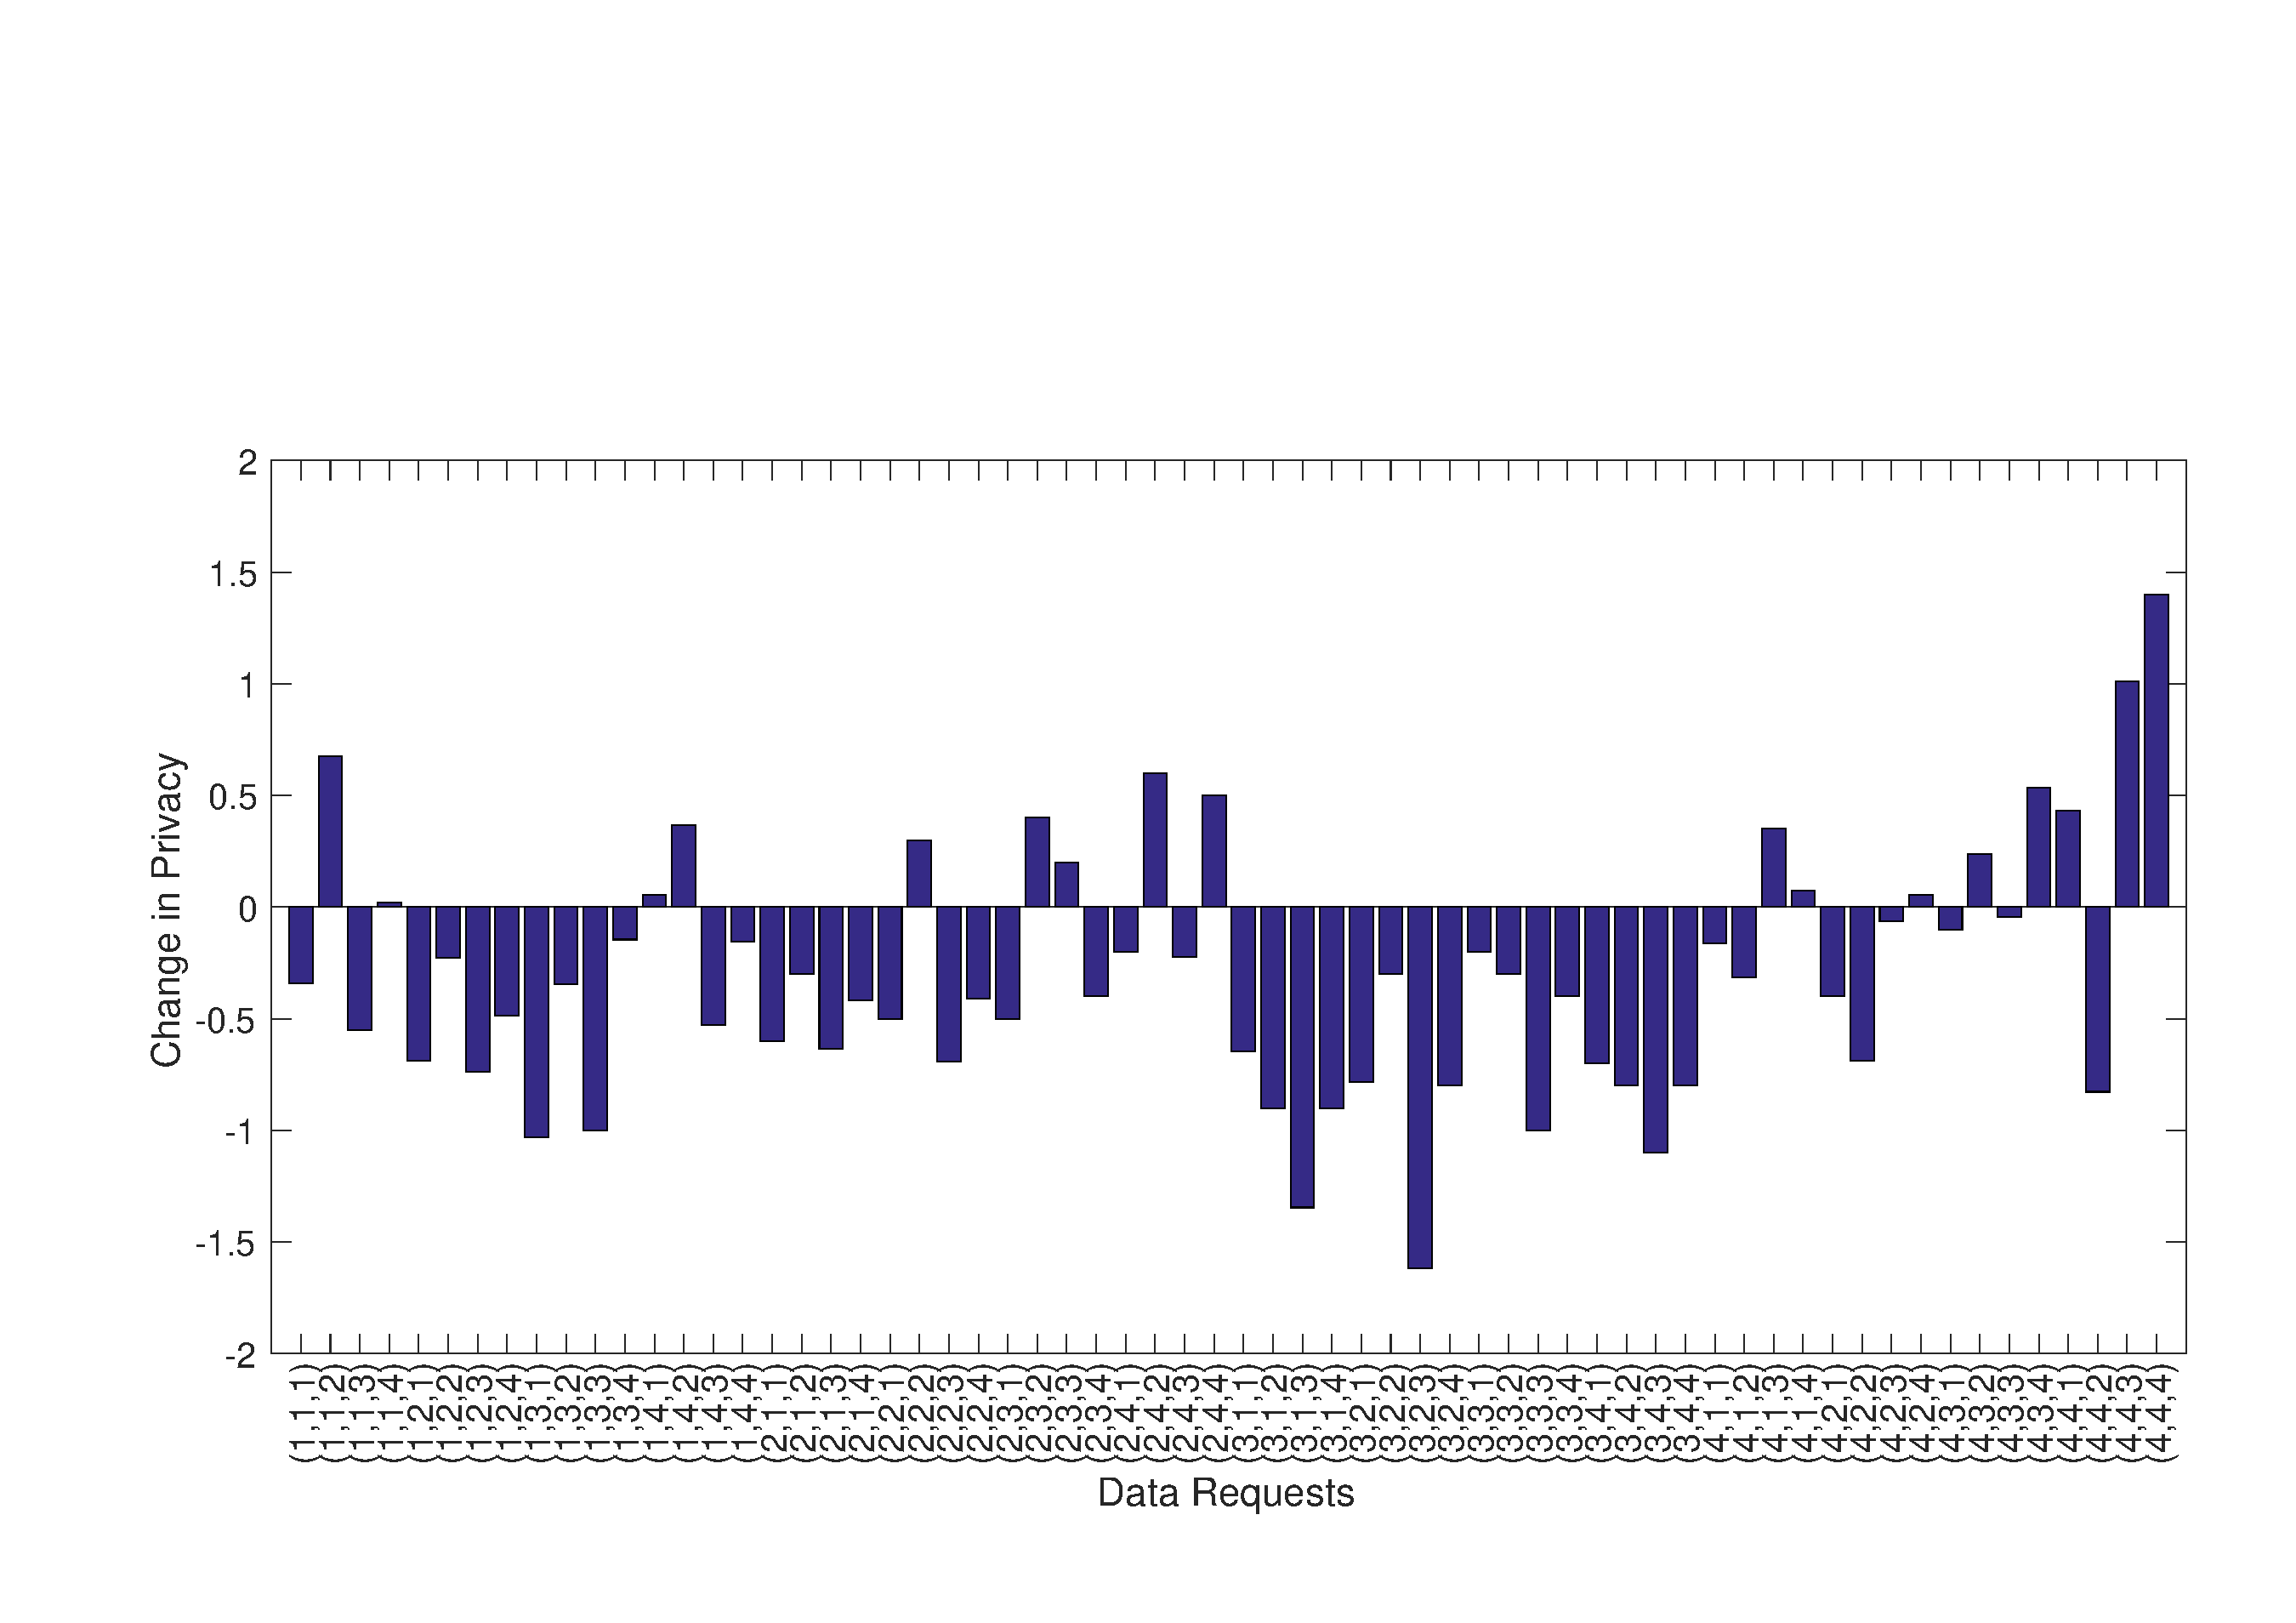
\includegraphics[width=\textwidth,keepaspectratio]{./images/day2_day1_privacy}
\caption{Gain in Privacy Between Day 2 and Day 1}
\label{fig:day2_day1}
\end{figure}

Figure \ref{fig:day2_day1} depicts the gain in privacy for day 2 compared to day 1. In day 2, incentives were given for data requests whereas in day 1 no incentives were given. The x-aixs depicts each data request with a sensor identifier, a stakeholder identifier and a context identifier. For detailed explanation as to which feature belongs to which identifier please refer section \ref{struct}. 

As observed, it is seen that for most data requests the privacy is negative which means users chose lower summarization levels to gain more credit. Similarly, figure \ref{fig:day3_day1} depicts the gain in privacy for day 3 compared to day 1. In day 3, incentives were given for data requests whereas in day 1 no incentives were given. Here as well it is seen that users have chosen to improve their credit compared to day 1. 

In day 3, more of the users are responding to incentives as it is seen that there are lesser bars on the positive side of privacy compared to day 2. This can be because users were getting used to the application interface and were more explorative on the second day to see changes in privacy and credit metrics. Additionally, it is also observed that the bars in the negative side in day 3 are smaller than day 2. This can be because users may be expecting even higher rewards for day 3 of the experiment than day 2, but still wanted to improve their credit.

\begin{figure}[ht!]
\centering
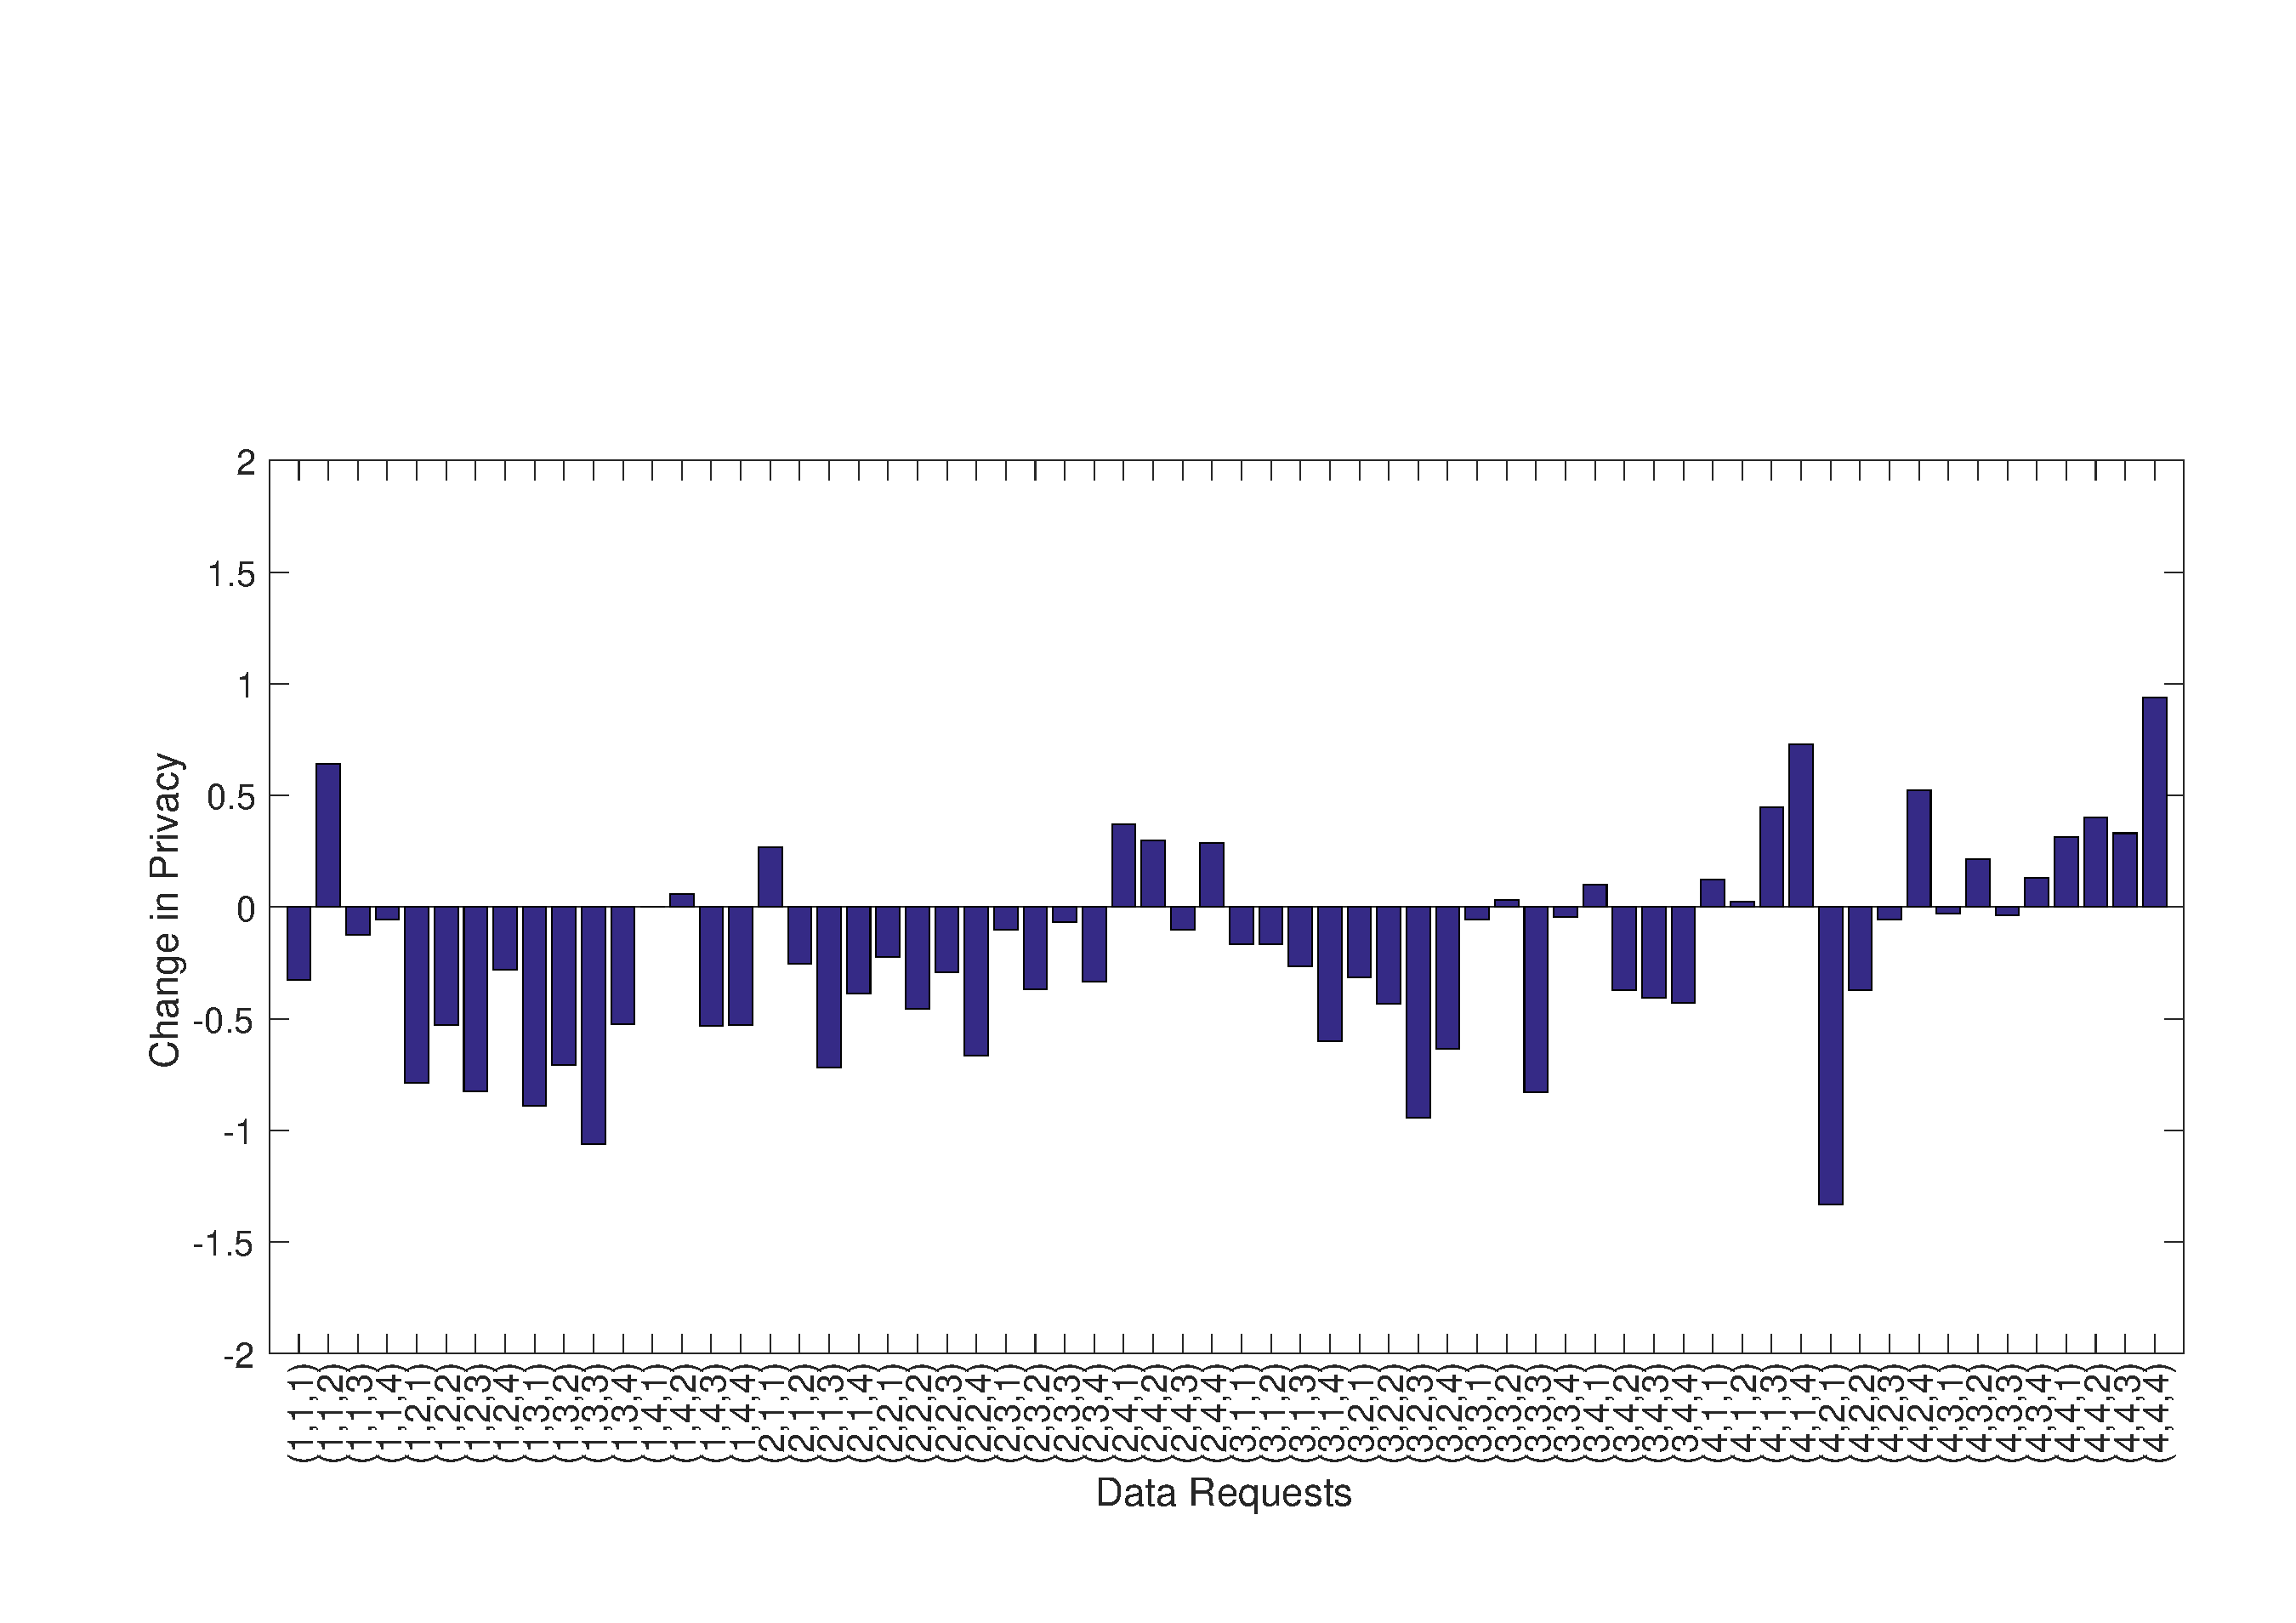
\includegraphics[width=\textwidth,keepaspectratio]{./images/day3_day1_privacy}
\caption{Gain in Privacy Between Day 2 and Day 1}
\label{fig:day3_day1}
\end{figure}


Figure \ref{fig:day3_day1} shows that for the location sensor (all tuples starting with 4), users were not icentivized enough. In general, it is observed that for stakeholders corporation and educational institution ( data requests (*,1,*) and (*,4,*) respectievely) users chose higher privacy levels. Even tough on an average users categorized educational institution as 3.29 on five which was the second least intrusive stakeholder, they still did not share more data possibly because of their affiliations with the department. It can also be that the privacy metric made users aware about the amount of data given to stakeholders and made them more privacy concious.

*** (Comparison of privacy intrusion levels of features compared to the pre survey graph yet to be added) ***



